\documentclass[a4,center,fleqn]{NAR}
%\usepackage{biblatex}
%\usepackage[
%backend=biber,
%style=alphabetic,
%sorting=ynt
%]{biblatex}
%\addbibresource{swissrepeat_literature.bib} %Imports bibliography file
%\usepackage{todonotes}
% orange = formatting
% red = TRs
% blue = homorepeats
% green = IDP
\usepackage{subcaption}
\renewcommand{\thesubfigure}{\Alph{subfigure}} % Capital letters for Subfigures
\usepackage{graphicx}
\graphicspath{{/home/matteo/polybox/MSc_ACLS/swissrepeat/}}

\usepackage{cleveref}
\usepackage{makecell}
\usepackage{lmodern} % For support of italic text, bold section-headers and modern formatting of abstract and title




% Enter dates of publication
%TODO
\copyrightyear{2019}
\pubdate{13 February 2019}
\pubyear{2019}
\jvolume{1}
\jissue{1}


%\articlesubtype{This is the article type (optional)}

\begin{document}

\title{A new Census of Protein Tandem Repeats and their Relationship with Intrinsic Disorder}
%\title{A new Census of Protein Tandem Repeats: Fun with Disorder.}

\author{%
Matteo Delucchi$^{1,2}$,
Elke Schaper$^{3}$,
Oxana Sachenkova Lundstr\"om$^{4,5}$,
Arne Elofsson$^{4}$,
and Maria Anisinova$^{1,2}$
\footnote{Dr. Maria Anisimova, ZHAW School of Life Sciences and Facility Management, Institute for Applied Simulations, Computational Genomics, Tel: +41 (0)58 9345882; Email: maria.anisimova@zhaw.ch}}

\address{%
$^{1}$, ZHAW W\"adenswil, Switzerland 
$^{2}$, Swiss Institute of Bioinformatics, Lausanne, Switzerland 
$^{3}$, Currently at Carbon Delta AG, Switzerland 
$^{4}$, Stockholm University, Stockholm, Sweden 
$^{5}$, Currently at Aiwizo AB, Stockholm, Sweden   
}
% Affiliation must include:
% Department name, institution name, full road and district address,
% state, Zip or postal code, country

\history{% 
%TODO fix dates.
Received January 1, 2009;
Revised February 1, 2009;
Accepted March 1, 2009}

\maketitle

\begin{abstract} %max 200 words
%TODO Maria: rewrite abstract
%We analyze systematically and with state of the art methods all known protein sequences for adjacently repeated amino acid sequence patterns.
We analyze systematically and with state of the art methods all known protein sequences for tandem repeats.
From all curated proteins of all domains of life, 50.9\% contained at least one tandem repeat. Eukaryotic proteins tend to have more TRs than prokaryotic which could be explained by the complexity of the respective organisms. 
A positive linear correlation between the amount of TR units and protein length could be detected. This correlation becomes weaker with increasing TR unit size.
TRs often didn't appear alone in the same protein. 43\% of eukaryotic proteins have even more than four distinct TR per protein. We further saw that small TRs appear more frequently and we showed that TRs are non-uniform distributed across the protein sequence. They are mostly located towards the ends.
We provide insights in the origin and function of proteomic tandem repeats across all kingdoms of life.
\end{abstract}


\section{Introduction}
The continued progress in genomics demands better classification and understanding of genomics sequences, their evolution and function across the tree of life. 
Proteins indisputably remain at the heart of the molecular machinery performing a multitude of essential functions. 
%%%%%%%%%%%%%%%
%%% TR Description & Terminology
%%%%%%%%%%%%%%%
According to most recent estimates a substantial amount of proteins contain adjacently repeated amino acid (AA) sequence patterns, known as tandem repeats (TRs).  
TRs are described by the length of their repeating motif (unit length), the number of repeated units (size) and the similarity among their units \cite{Schaper2015} (see figure \ref{fig1_TRsketch}). \\
TRs are highly abundant in human proteome $>55\%$ \cite{Rollins2005} and display an impressive variability of sizes, structures and functions \cite{Schaper2012, Schaper2014}. 
Proteins containing TRs have enhanced binding properties \cite{Li2003} and are known to have associations with immunity related functions \cite{Usdin2008, Madsen2008} and diseases.
%TODO add more REFs here. See Discussion for references
As an example, unamyotrophic lateral sclerosis, myotonic dystrophy, dentatorubral-pallidoluysian atrophy, frontotemporal dementia, fragile X syndrome, fragile X tremor-ataxia syndrome, Huntington disease, spinobulbar muscular atrophy and spinocerebellar ataxia are all caused through tandem repeat disorders (TRD) \cite{Hannan2018}. \\
% **************************************************************
% Keep this command to avoid text of first page running into the
% first page footnotes
\enlargethispage{-65.1pt}
% **************************************************************
%%%%%%%%%%%%%%%
%%% TR evolvement/building mechanism
%%%%%%%%%%%%%%%
Similarity between the TR units fades with time since TRs can evolve either during meiosis or mitosis by processes such as duplication and loss of TR units, recombination, replication slippage and gene conversion which all can cause changes to their unit similarity and length \cite{Ellegren2004}. This evolution in TR units makes them a rich source for genetic variability by providing a wide range of possible genotypes at a given locus \cite{Nithianantharajah2007}. Therefore, they are prone to selection on long evolutionary scales as well as on a somatic level. The occurrence of mutations in TR within protein coding genes, can alter the structure and therefore likely the function of the affected protein too. Since non-coding regions play crucial roles in gene regulation, transcription, and translation, the proteins concerned are also likely to be affected by mutations occurring in non-coding TRs.
%TODO Mars paper?
While the biological mechanisms generating TRs are not well understood, evidence suggests that natural selection contributes to shaping TR evolution \cite{Schaper2014},
%(REFs: Mar’s paper 
and that TR expansion is linked to the origin of novel genes \cite{Light2014}
TRs have been successfully exploited in bioengineering due to their “design-ability” \cite{Javadi2013}.

%\begin{figure*}[ht]
%\centering
%\begin{subfigure}{.5\textwidth}
%  \centering
%  \includegraphics[width=0.9\textwidth]{{paper/TR_scetch/TR_classification_scetch.png}}
%  \caption{}
%  \label{figSketchTR}
%\end{subfigure}%
%\begin{subfigure}{.5\textwidth}
%  \centering
%  \includegraphics[width=0.9\textwidth]{{paper/figures/fig1.png}}
%  \caption{}
%  \label{fig1}
%\end{subfigure}
%\caption{(A) A sketch of a tandem repeat with it's descriptors. This micro TR with the ID A7TKR8 and a size of 6 units, each with a unit length of 3 amino acids shows a head-to-head orientation and consists of mixed units - a direct- and heterorepeat.
%(B) Distribution of all annotated TRs as a function of their repeat unit length $l_{effective} <= 80$ and their number of repeat units $n_{effective} <= 40$. Darker colour indicates a larger number of TRs with a specific length and number of repeats. The majority of TRs has small TR units. Yet, there is a blob of domain TRs ($25 < l_{effective} < 50$), with certain TR unit length clearly enriched (e.g., $l_{effective} = 28$, mostly zinc finger TRs.)}
%\end{figure*}

\begin{figure*}[t]
\begin{center}
\includegraphics[width=0.75\textwidth]{{paper/figures/fig1_TRscetch_labeled.png}}
\end{center}
\caption{(A) A sketch of a tandem repeat with it's descriptors. This micro TR with the ID A7TKR8 and a size of 6 units, each with a unit length of 3 amino acids shows a head-to-head orientation and consists of mixed units - a direct- and heterorepeat.
(B) Distribution of all annotated TRs as a function of their repeat unit length $l_{effective} <= 80$ and their number of repeat units $n_{effective} <= 40$. Darker colour indicates a larger number of TRs with a specific length and number of repeats. The majority of TRs has small TR units. Yet, there is a blob of domain TRs ($25 < l_{effective} < 50$), with certain TR unit length clearly enriched (e.g., $l_{effective} = 28$, mostly zinc finger TRs.)}
\label{fig1_TRsketch}
\end{figure*}


\subsection{A Comprehensive Analysis of Proteomic Tandem Repeats}
Despite much interest \cite{DiDomenico2013}, the most recent and commonly cited census of protein TRs summarizing repeats from UniProtKB/Swiss-Prot protein knowledgebase \cite{UniProt2017} dates back two decades \cite{Marcotte1999}. Since then the number of proteins in the curated protein data bank SwissProt has grown more than seven fold (\ref{sup:figSwissProtStats}).
Equally, a multitude of new methods were developed for the prediction and analysis of TRs \cite{Anisimova2015, Fertin2015, Dashnow2018}. In particular, due to striking differences in TR predictor properties, a new statistical framework and a meta-prediction approach was proposed in order to increase the accuracy and power of the TR annotation \cite{Anisimova2015, Schaper2015}.\\
%%%%%%%%%%%%%%%
%%% The idea about this paper
%%%%%%%%%%%%%%%
Here we apply this recent methodology to characterize the distribution of protein TRs as found in the up-to date SwissProt protein knowledgebase \cite{Boutet2016, UniProt2017}. Our TR annotation for each protein includes the TR region start, end, minimal repeated unit length, among unit divergence and TR unit alignments. This allows our study to provide an unprecedented detail of the universe of protein TRs.\\
%TODO check for REFs
%%%%%%%%%%%%%%
%%% Virus virus-host interaction
%%%%%%%%%%%%%%
To our knowledge, no recent study connected the information of viral proteomic TRs to their hosts TRs. 
Viral genomes are generally relatively small which demands for an optimal coding capacity. 
%Smaller proteins are less likely to contain many TRs. 
Furthermore, they lack their own translational apparatus and depend completely on their hosts protein synthesis machinery \cite{Walsh2003, Stern2018}. This makes them an interesting subject of research and therefore we provide a large-scale study of viral TRs comparing the TR distributions of viral and their hosts proteomes.\\
%We therefore investigated whether we see any common characteristics and correlations between the proteomic TRs of viruses and their corresponding host organisms. 
%%%%%%%%%%%%%%
%%% IDR
%%%%%%%%%%%%%%
Proteins with TRs tend to be enriched with intrinsic protein disorder (IDP) \cite{Jorda2010}, and vice versa \cite{Szalkowski2013}.
%further REFs
IDPs cover multiple three dimensional states of proteins leading to different functionalities \cite{Dunker2001}. 
%TODO more REFs
Both TR and intrinsic disordered regions (IDR) also tend to be over represented in the hubs of protein-protein interaction networks \cite{Ekman2006}. While the relationship between these non-globular protein features has been observed, the biological reasons are not well understood. 
TRs often fold into specific structures, such as solenoids, or have “beads on a string” organizations \cite{Kajava2012}. But there is undoubtedly a class of protein TRs strongly associated with unstructured regions \cite{Jorda2010, Szalkowski2013}. Several studies have shown that compositionally biased, low complexity regions often found in IDPs, evolve rapidly, including recombinatorial repeat expansion events \cite{Tompa2003, Simon2009}. Others in contrast observed that the association between repeat enrichment and protein disorder is not as clear \cite{Light2013}.
In order to systematically characterize and explore the enigmatic connection between TRs with IDP, we also use state of the art methods to annotate each protein with IDP regions and summarize the distribution of the overlap of TR and intrinsic disordered regions over all kingdoms of life. 
This characterisation of overlaps with offers an unprecedented detailed view of the interplay of TRs with IDR. 

\section{RESULTS}
Exhaustive annotation of protein TRs in the entire UniProtKB/Swiss-Prot was done using a meta-prediction approach based on both de novo and profile-based methods followed by filtering of false positives and redundancies. The pipeline was implemented in Python using TRAL \citep{Schaper2015}; see Methods for details. Structural and biochemical properties of TRs can be extremely diverse depending on the length and the composition of their minimal repeating unit. We studied TR properties in four categories defined according to TR unit length L:
(1) homorepeats $L=1$, (2) microrepeats $1 < L \leq 3$, (3) small repeats $4<L\leq15$, and (4) domain repeats $\geq 15$. 

%%%%%%%%%%%%%%
% Amount of TRs
%%%%%%%%%%%%%%
Predicted TR annotations and their distributions with respect to protein length and repeat number are summarized by superkingdoms \cite{Nasir2012} in table \ref{tab:No_of_TR_annotations} and in the figures \ref{sup:figTR_distribution_unit_number} and \ref{sup:figTR_distribution_unit_length}.
% \ref{figTR_distribution_unit_length} and \ref{figTR_distribution_unit_number} respectively. 

\begin{table*}[]
\tabcolsep=0.1cm
\begin{tabular*}{\textwidth}{@{\extracolsep{\fill}}llrlll@{}}
  \hline
  \\[-0.75em] % rowpadding: 0 huge padding; -1 no padding
all proteins & Archaea & Bacteria & Eukaryota & Viruses\\ 
  \hline
  \\[-0.9em]
  protein count &  19370 & 332327 & 181814 &  16605 \\ 
  mean protein length & 288 & 313 & 436 & 451 \\ 
  TR count &   6420 & 103842 &  92472 &   7237 \\ 
  TR fraction & 0.331 & 0.312 & 0.509 & 0.436 \\ 
  \;\;\;homo TR & 0.006 & 0.006 & 0.086 & 0.029 \\
  \;\;\;micro TR & 0.117 & 0.109 & 0.245 & 0.191 \\ 
  \;\;\;small TR & 0.217 & 0.208 & 0.328 & 0.300 \\ 
  \;\;\;domain TR & 0.051 & 0.049 & 0.143 & 0.069 \\ 

  \hline
  \\[-0.75em]
proteins containing TRs   &   &   &   &   \\ 
  \hline
  \\[-0.9em]
  mean protein length & 355 & 404 & 572 & 644 \\ 
  mean TR length & 9.9 & 9.4 & 10.8 & 7.6 \\
  TR fraction &   &   &   &   \\ 
  \;\;\;homo TR & 0.019 & 0.019 & 0.169 & 0.067 \\
  \;\;\;micro TR & 0.354 & 0.350 & 0.482 & 0.438 \\ 
  \;\;\;small TR & 0.656 & 0.667 & 0.644 & 0.689 \\ 
  \;\;\;domain TR & 0.154 & 0.157 & 0.281 & 0.158 \\ 
  \hline
\end{tabular*}
\caption{Swiss-Prot entries by kingdoms for all proteins and for proteins that contain TR.
The total amount of proteins per superkingdom is given as \textit{protein count}. \textit{TR count} refers to the number of proteins which contain at least one TR. 
Over all proteins, Bacteria has the most entries but Eukaryota the biggest fraction of proteins with TRs and also the longest TRs. Viruses tend to have the longest protein sequences - with or without TRs; followed by eukaryotic and prokaryotic proteins.
In general, small TRs prevail over the other types. }
\label{tab:No_of_TR_annotations}
\end{table*}
% To make table pagewidth/textwidth: https://tex.stackexchange.com/questions/336288/nar-latex-template-paperwide-table

\subsection{TRs are Abundant in Proteins of all Domains of Life}
Overall, 50.9\% of all eukaryotic proteins contained at least one TR:
In \textit{Homo sapiens} (Human), 68.8\%, \textit{Mus musculus} 61.9\%, \textit{Drosophila melanogaster} 60.8\% and in  \textit{Escherichia coli} 28\% of all proteins contain TRs. 
%TODO mention this next sentence?
%A more detailed view is given in figure  \ref{sup:figPerc_TRs_all_sp_prots} where the percentage of proteins containing at least one TR is plotted against the average length of the proteins per species.
%TODO [There were interesting examples in Jorda \& Kajava 2010, although just for homorepeats.] 
Interestingly, 43.6\% of viral proteins contained TRs, almost as frequently as in Eukaryotes. In comparison, fewer prokaryotic proteins contained TR, but nevertheless >30\% for both bacterial and archaeal proteins. 

%%%%%%
%%% homo TRs
%%%%%%
Proteins containing homo TRs have generally TRs mostly of small size (mean = 8.8 units). They make up 20\% of all annotated TRs over all superkingdoms and 30\% for human TRs. Of all the homo TRs, 91.3\% are of eukaryotic origin. We couldn't detect a protein which contains only homo TRs and no other type of repeat.
%TODO human Homorepeats are well known for their disease association.

%%%%%%
%%% micro TRs
%%%%%%
Proteins with micro TRs tend to have TRs with a mean of 7 repeat units. For proteins which contain only micro TRs, the mean repeat unit number = 3. 
Proteins containing micro TRs make up 56\% of all annotated TRs.

%%%%%%
%%% small TRs
%%%%%%
Proteins with small TRs tend to have TRs with less repetition units than those with homo TRs (mean = 6 units). For proteins which contained solely small TRs, the mean unit number is 3. 
Proteins containing small TRs make up 76\% of the found TRs.

%%%%%%
%%% domain TRs
%%%%%%
Domain TRs mostly consist of few units (mean = 3.5 units). A prominent exception is an extracellular matrix-binding protein (Q5HFY8, \textit{S. aureus}) with ~80 units each ~97aa (PF07564) spanning ≥7700aa. Other examples of bacterial domain TRs with many units are the cell surface glycoprotein 1 of \textit{Clostridium thermocellum} and uncharacterized PE-PGRS family proteins of \textit{Mycobacterium tuberculosis} with $> 300$ units and a TR length of up to 1707aa. Proteins containing domain TRs make up 30\% of all predicted TRs.

Eukaryotic domain TRs tend to be more uniformly distributed in terms of their TR size. The proteins with the most repeat units belong to mediator of RNA polymerase II transcription subunit proteins from yeast (\textit{{Eremothecium gossypii}}), slime mold (\textit{{Dictyostelium discoideum}}) and human Mucin-22 protein.
Figure \ref{sup:figTR_distribution_unit_number} shows a peak of proteins containing many TR units. They seem to belong to collagen-like proteins of the Mimiviridae family.

\subsection{TRs vary in their Length and Number}
%%%%%%%%%%%%%%
% TR unit length vs TR unit number
%%%%%%%%%%%%%%
In general, TRs are not homogeneously distributed in terms of their unit lengths and numbers. Figure \ref{fig1_TRsketch} reveals multiple peaks, showing that some unit lengths are particularly frequent. These peaks represent common TRs, with specific TR units used in varying number.  
One such example are zinc finger proteins, abundantly present as a TR in all domains of life, but also LRR and WD40-like beta propeller.

In Bacteria (\textit{Porphyromonas gingivalis}) hemagglutinin A is known to be involved in host colonisation by adhesion to extracellular matrix proteins and is expected to be involved in periodontal diseases \cite{Nelson2003, Han1996}. 
It can be seen in figure \ref{sup:figTR_distribution_unit_length} as one of the bacterial outliers (in terms of unit length) with a unit length $>450$. The other two outliers belong to the Mannuronan epimerase protein of \textit{Azotobacter vinelandii}.
Eukaryotes tend to have in general the longest TR units with strong outliers which belong to the Anchorage 1 protein and Nesprin homolog in \textit{Caenorhabditis elegans} and Mucin-12 
%MUC12 A gene on chromosome 7q22 that encodes an epithelial mucin belonging to a family of secreted and cell surface glycoproteins, involved in epithelial cell protection, adhesion modulation and signalling. MUC12 may be involved in epithelial cell growth regulation, and is stimulated by both cytokine TNF-alpha and TGF-beta in intestinal epithelium.
and FC$\gamma$BP (which has mucin-like structure \cite{Harada1997}) in humans. 

\subsection{Multiple Tandem Repeats per Protein}
%%%%%%%%%%%%%%
% more than one distinct TR region
%%%%%%%%%%%%%%
A substantial fraction of proteins contained more than one distinct TR region, most frequently in eukaryotic proteins (56\% of all proteins with TRs), but also in viral (45.7\%) and prokaryotic proteins (28.4\% in Bacteria and 26.6\% in Archaea). 
In Eukaryotes, 43\% (90026 absolute count) of all proteins with TRs had 4 (or more) distinct TR regions. After them come Viruses with 28.6\% followed by Bacteria 9.1\% and Archaea with 8.0\% having $\geq 4$ distinct TR regions per protein.

In proteins which have $\geq 4$ TRs, the TR-types are not necessarily the same. 
%TODO reason this explicitly.
By far the most frequent TRs in proteins containing $\geq 4$ TR regions, were small repeats (95.0\% of all predicted TRs), followed by microrepeats (87.9\%), and domainrepeats (47.6\%) (\ref{sup:figTRtypes_distribution_in_prot_with_more_4TRs}).

\subsection{More TRs are Found in Longer Proteins}
%%%%%%%%%%%%%%
% Protein Length vs TR fraction
%%%%%%%%%%%%%%
Proteins with a chloroplastic origin tend to be shorter and contain less TR than Viridiplantae proteins from mitochondrial origin. Mitochondrial proteins are in general shorter and have less TR than proteins without endosymbiontic origin.
Figure \ref{figPerc_TRs_all_sp_prots_all} displays the linear relationship between mean protein length and the amount of TR. Prokaryotic proteins cluster with their protein length and TR content in the same range as chloroplastic proteins. 
%TODO endosymbiontic theory!
It seems that TRs are increasingly abundant in increasingly complex organisms (consider also figure \ref{sup:figPerc_TRs_all_sp_prots}). 
%TODO compare to IDRs which are the same: increasingly abundant in increasingly complex orangisms!

\begin{figure*}[ht]
\centering
\begin{subfigure}{.5\textwidth}
  \centering
  \includegraphics[width=0.9\textwidth]{{paper/figures/Mean_Prot_length_vs_Frac_TR.png}}
  \caption{}
  \label{figPerc_TRs_all_sp_prots_all}
\end{subfigure}%
\begin{subfigure}{.5\textwidth}
  \centering
  \includegraphics[width=0.9\textwidth]{{paper/figures/fig2a-2.png}}
  \caption{}
  \label{fig2a-2}
\end{subfigure}
\caption{(A) The fraction of proteins containing TRs over all protein entries in UniProtKB/Swiss-Prot is shown for each taxonomic domain (superkingdom) or kingdom and displayed as function of the mean protein length and split according to the origin of the proteins.
Chloroplastic proteins seem to be shorter and tend to have less TR than mitochondrial proteins. Non-mitochondrial and non-chloroplastic proteins appear to be longer and with more TRs.
(B) The fraction of proteins with TRs as a function of sequence length by kingdom resulting in a linear relationship. With Eukaryotes having on average more TRs than the other kingdoms.}
\end{figure*}


A different level of detail is obtained by not only considering the mean of the protein length, but by grouping the amount of TRs according to bins of protein sequence length.
Figure \ref{fig2a-2} shows that in general, differences in TR distributions observed between kingdoms can be largely attributed to protein sequence length with Eukaryotes having on average longer TRs.
The fraction of eukaryotic proteins with homo TRs behaves differently than in other TR-types and compared to the other superkingdoms: The amount of homo TRs in eukaryotic proteins increases exponentially whereas for the other superkingdoms, the homo TR fraction remains similar with increasing protein length (\ref{sup:fig2a-3}, \ref{sup:fig2a-4}, \ref{sup:fig2a-5}, \ref{sup:fig2a-6}).
Looking specifically at proteins which contain TRs, we can see in figure \ref{sup:fig2a} that on average longer protein sequences tend to have more TRs and small TR seem to be the most recurrent in all kingdoms.
%TODO explanation why? -> PFAM? see notebook p.46

Indeed, we observe a positive correlation between the protein length and the fraction of proteins with TRs across all kingdoms of life for all TR types: 
$R^2 = 0.46, \; p<0.001$ for homo TRs;
$R^2 = 0.64, \; p<0.001$ for micro TRs; 
$R^2 = 0.88, \; p<0.001$ for small TRs, and 
$R^2 = 0.24, \; p=0.08$ for domain TRs.

The lack of correlation for domain TRs, where factors other than protein length must contribute to explain the amount of TRs, could be explained through differences in TR generating processes for different TR types and that they are like architectural blocks performing certain functions on their own. On the other hand, consistent with the same trend, we observed that homorepeats are particularly frequent in Eukaryotes, where proteins are on average longer. Moreover, longer homorepeats are mostly characteristic to eukaryotic proteins. For example, this can be observed in figure \ref{fig5a}. PolyQ and polyN homorepeats may often be observed with $>50$ repetitions in Eukaryotes. The same homorepeats display $<10$ repetitions for polyQ and $<20$ for polyN in Prokaryotes and Viruses. However, this large discrepancy cannot be explained purely by the length of the proteins involved. 
%TODO [Can we back this up or reject? for example, can we compare the extent of differences of protein lengths with polyN and polyQ (separately) for eukaryotes vs. other?]

\begin{figure}[t]
\begin{center}
\includegraphics[width=0.5\textwidth]{{paper/figures/fig5a.png}}
\end{center}
\caption{Count of homorepeats in Swiss-Prot in four superkingdoms for different repeat unit number ($n <= 50$, equivalent to repeat length) for hydrophilic Asparagine (N), Glutamine (Q), Serine (S) and Glutamic acid (E). Homorepeats with large $n$ seem to mostly pertain to the Eukaryotes. }
\label{fig5a}
\end{figure}

%\begin{figure}[t]
%\begin{center}
%\includegraphics[width=0.5\textwidth]{{paper/figures/fig2b.png}}
%\end{center}
%\caption{TMean disorder content as a function of sequnce length. [Note: how much complexity should we show?]}
%\label{fig2b}
%\end{figure}
%
%\begin{figure}[t]
%\begin{center}
%\includegraphics[width=0.5\textwidth]{{paper/figures/fig2b_simple.png}}
%\end{center}
%\caption{Mean disorder content as a function of sequnce length. [Note: how much complexity should we show?]}
%\label{fig2b-simple}
%\end{figure}

\subsection{TR-location is Biased Towards Flanks for Shorter TRs}
%%%%%%%%%%%%%%
% TR location
%%%%%%%%%%%%%%
Next, we explored where in a protein sequence tandem repeated regions tend to be found. The location within a protein was evaluated with respect to the center of a TR region and normalized by the protein length (see Methods).  
The observed distribution of TRs along the protein length was non-uniform and dependent on the TR unit length. Figure \ref{sup:fig3a_all_renormalized} shows the distributions of the relative positions of TRs in proteins across all different kingdoms and for different TR unit length categories.

As expected, TR relative position is preferably near to the start of protein sequences.  For homorepeats such tendency was particularly striking, particularly in Archaea, where most homorepeats were found in the C-terminal and domain TRs which tend to be found at the N-terminal (\ref{sup:figTR_position_all_by_Superkingdom}).
Overall, shorter TRs (homo, micro and small) displayed stronger preferences towards both, N- and C- terminals of proteins. 
%TODO [Again any special cases could be mentioned here. For example in viruses we see a blue spike towards the C-terminal. Does this correspond to any special features of viruses also see in the figure 1, for some specific TR? ]
%TODO [ToDo: Potentially compare to random distribution. Or, normalize by "first possible occurrence", instead of "sequence length".]
In particular for Eukaryotes, there was a clear correlation between the TR unit length and the location bias towards the protein flanks. 
Interestingly, also domain TRs in Viruses and to a smaller degree in Archaea show a similar behavior to be located towards both flanks of proteins.
%Interestingly, also domain TRs in Viruses and to a smaller degree in Archaea show a similar behavior to be located towards both flanks of proteins, notwithstanding, our findings are based on a relatively limited number of observations (1290 and 955 respectively), the results from such analyses should thus be treated with caution.
%TODO put the warning in discussion?
In eukaryotic proteins TRs were found to be overrepresented in the N-terminal protein flank, while in Archaea and Bacteria, the TR preference was towards the C-terminal. 


%%%%%%%%%%%%%%
% Disorder location
%%%%%%%%%%%%%%
Analogously we looked at the location of IDRs in proteins and found parallels to TRs. IDRs tend to be located towards the flanks, while short IDRs tend to be located near the N-terminal, see fig. \ref{sup:fig3b}. 

\subsection{TRs Are Enriched With Disorder Promoting Amino Acids}
%\subsubsection{TR and disorder overlap is mostly explained by skewed amino acid frequencies}
Further we evaluated the abundancy of amino acids in TRs with respect to their disorder-promoting propensity \cite{Uversky2013}.

The amino acid abundances in TRs are linear dependent to their respective abundances in proteins (fig. \ref{AA_ratio}).
TRs can not be characterized by a certain amino acid abundancy pattern.
However, we could find a significant positive correlation ($\rho = 0.71,\; p < 0.05$) of the abundancy of amino acids in TRs with the corresponding amino acid's disorder propensity (\ref{sup:AA_ratio_facet}). In contrast, the overall amino acid abundancy in all proteins (incl. TR-containing) showed much lower correlation and significance ($\rho = 0.44,\; p = 0.053$). We couldn't detect any correlation when the TR-containing proteins were excluded from the overall fraction ($\rho = -0.10,\; p > 0.05$).

\begin{figure}[t]
\begin{center}
\includegraphics[width=0.5\textwidth]{{paper/figures/AA_ratio_TR_vs_background.png}}
\end{center}
\caption{AA frequencies in tandem repeats against the amino acid frequency over all proteins normalized by their total amount of amino acids. An increased size of the dot corresponds to an increased disorder propensity. The distribution of the AAs in TRs corresponds to the overall distribution in proteins eliminating a distribution bias.}
\label{AA_ratio}
\end{figure}

%TODO show this in suppl.? NOTE: I don't know how the disorderlength was calculated though!
%\subsection{Localization of TRs and disorder.}
%\begin{figure}[t]
%\begin{center}
%\includegraphics[width=0.5\textwidth]{{paper/figures/fig4a.png}}
%\end{center}
%\caption{Shown is the fraction of disordered chars for micro TRs, small TRs and domain TRs. We see clearly bimodal distributions, with the majority TRs mostly ordered, however with a striking fraction of small TRs and micro TRs mostly disordered.}
%\label{fig4a}
%\end{figure}

%%%%%%%%%%%%%%
% empirical homo repeats
%%%%%%%%%%%%%%
In homo TRs, grouped by their presence in disordered or ordered regions, figure \ref{fig5c}) shows that amino acids which were expected to promote disorder, appear more often in homo TRs of AA with a higher disorder promoting propensity. 
%TODO discussion: Does it allow to conclude, that high disorder propensity relates to high repeat unit number?
In Eukaryotes, homo TRs were longer compared to the other superkingdoms (\ref{sup:fig5a}).
%TODO discussion: this is becase especially polyN an polyQ repeats are known to be involved in the protein structure relevant for protein-protein interaction 
In general we observe an exponential decay 
%TODO ask maria
%[TODO: The scale is log10. Can we still say exp.-decay?] 
of homo TRs with increasing repeat unit number except for polyhistidine (polyH), polyasparagine (polyN) and polyglutamine (polyQ).
PolyN and polyQ homo TR frequently appear to be longer compared to the other residues. 
We further see that polyN and polyH homo TR which have a low disorder promoting propensity, appear relatively frequent as long repeats.

\begin{figure*}[ht]
\centering
\begin{subfigure}{.5\textwidth}
  \centering
  \includegraphics[width=0.9\textwidth]{{paper/figures/fig5c.png}}
  \caption{}
  \label{fig5c}
\end{subfigure}%
\begin{subfigure}{.5\textwidth}
  \centering
  \includegraphics[width=0.9\textwidth]{{paper/figures/fig5b.png}}
  \caption{}
  \label{fig5b-2}
\end{subfigure}
\caption{(A) Empirical count of homorepeats in Swiss-Prot Eukaryotes ($n <= 50$) for ordered and disordered regions (consensus MobiDB annotations, no minimum length cut-off). Amino acids are ordered by their propensity to promote structural order. It can be seen, that polyN and polyH regions, are frequently detected within disordered protein regions even though their disorder promoting propensity is relatively low. Further, the frequency of polyQ and polyN residues decreases differently with increasing length, than for other AA.
(B) Empirical and expected count of homorepeats in Swiss-Prot Eukaryotes ($n <= 50$). Amino acids are ordered by their propensity to promote structural order. It can be observed, that disorder promoting residues are found more often than expected in long TRs. PolyN and polyH repeats have a low disorder propensity but show the characteristics observed in AA with high disorder propensity.}
\end{figure*}



%%%%%%%%%%%%%%
% expected homo repeats
%%%%%%%%%%%%%%
To compare the empirical observations with statistical expectation, we estimated the number of homo TRs of a certain amino acid and repeat unit number, (which corresponds to a sequential run of success in a Bernoulli trial; see Methods) and compared this to the observed number of homo TRs (fig. \ref{fig5b}).
Resulting in an exponential decay in frequency of homo TRs with increasing TR length.
This shows us, that disorder promoting amino acids appear more frequently in longer repeats than expected.

%CAVE: Be careful with interpretation because statistics of expected homo TRs doesn't take care of disorder propensity and regional and structural properties (structural properties of multiple dimensions)


\subsection{TRs in Intrinsic Disordered Regions}
To elaborate the association of TRs with IDR, we distinguish four types of overlap (\ref{sup:overlap_scetch}). We call the overlap a \textit{tail-overlap} where intrinsic disorder begins within the TR-sequence and finishes after the TR-region. In contrast, we call it \textit{head-overlap} if the IDR begins before the TR-sequence and finishes within. If the IDR lies completely within a TR sequence, we call it \textit{Disorder-in-TR} and \textit{TR-in-Disorder-overlap} if the TR-region lies within the IDR.
Only 9.1\% of residues in Swiss-Prot can be found in TR-regions, 12.9\% in intrinsic disordered regions and 2.5\% overlap.
Even though the overlap of TRs with IDRs is small, TRs and IDRs are frequently found in the same protein.
Intrinsic disorder regions are found in $27.8 \%$ of proteins with TRs whereas 19.6\% of the IDR overlap with TR regions. 
The largest fraction of overlap is due to a complete overlap of IDRs with TRs (fig. \ref{TR_disorder_overlap_overall_detail}) whereby TRs are mostly a complete part of IDR. 

\begin{figure}[t]
\begin{center}
\includegraphics[width=0.5\textwidth]{{paper/figures/TR_disorder_overlap_overall_detail_and_venn.png}}
\end{center}
\caption{(A) The absolute size of intrinsic disordered regions with TR-regions can be split in the four different kinds of overlap. We can see that TRs are most often nested within intrinsic disordered regions.
(B) The areas represent the total number of amino acids of each group. Where the rectangle shows the total amount of amino acids in all proteins, the amino acids in disordered regions and the amino acids in TR-regions and their overlap. 9.1\% of the length of protein sequences can be attributed to tandem repeated regions and 12.9\% to disordered regions. 2.5\% of the total length of protein sequences overlaps with both.}
\label{TR_disorder_overlap_overall_detail}
\end{figure}
%TODO supporting the idea that: "Approximately half of the tandem repeat regions has intrinsically disordered conformation being naturally unfolded.[5][6][7] " from wikipedia tandem repeats

\subsection{TRs are Involved in Transcription Processes, Structural Organisation, Electron-transport \& Ion-binding}
%\subsection{TRs are involved in a number of housekeeping proteins.}
%housekeeping proteins -> REF: Ferguson2005
From all detected TRs, 4.5\% were retrieved with a PFAM model. Clustering the PFAM model with the PFAM-Name we could associate TRs with their corresponding protein families (see methods for details). Many more entries for TRs with a PFAM entry could be detected in Eukaryotes (73\%) compared to the other superkingdoms.\\
%%%%%%%%%%%%%%
% TOP 10 PFAMs
%%%%%%%%%%%%%%
For each superkingdom, we filtered the 10 most frequently observed PFAM-families of TR containing proteins (whole list in suppl. table \ref{sup:PFAM_table}).
% These PFAM entries were then retrieved for all other superkingdoms too which allows us to observe the frequency of PFAM families accross superkingdoms. For the top-PFAM entries in TR containing proteins, we calculated their relative position in the proteins (see method for details). 
%%% Transcription
Which resulted in the overall detection of many TRs falling within proteins which are involved in transcription. 
As expected, in Eukaryotes many TRs in Zn-finger motifs were responsible for adhesion to DNA, RNA and lipids. WD-40 repeats inter alia involved in transcriptional regulation. RNA recognition motifs, such as the K Homology (KH) domain which binds to RNA, transcriptional repression such as the Pumilio-family, found in many TR-containing proteins in fungi. Eukaryotic proteins with TRs appear frequently to occur in  RNA-polymerase binding and RNA-splicing by i.e. KRAB box domain as well as proteins involved in the assembly of multiprotein complex.

%%% Electron-transport / Ion-binding
Additionally, many TRs were detected in proteins involved in electron-transport and ion-binding such as EF-hand domain pair and Ca\textsuperscript{2+}-binding EGF domain in Eukaryotes, the zinc-dependent enzyme UDP N-acetylglucosamine O-acyltransferase and the Rad50 zinc hook motif in Bacteria. Zinc-binding motifs could be detected in viral TR-containing proteins such as the zinc knuckle motif, too.

%%%%% Chloroplasts
In proteins of chloroplastic origin, we detected many TRs in NifU-like domains.
%http://www.ncbi.nlm.nih.gov/entrez/query.fcgi?cmd=Retrieve&amp;db=PubMed&amp;dopt=Abstract&amp;list_uids=11498000
%http://www.ncbi.nlm.nih.gov/entrez/query.fcgi?cmd=Retrieve&amp;db=PubMed&amp;dopt=Abstract&amp;list_uids=8875867
They are involved in the formation of metalloclusters of nitrogenase in certain bacteria and the maturation of FeS clusters. 

%%%%% Mitochondrion
Proteins from mitochondrial origin showed many TRs in proteins with EF-hand domain pairs which is found in a large family of Ca\textsuperscript{2+}-binding proteins and with Bacterial transferase hexapeptide which combines several transferase protein families including zinc metalloenzymes.
In both, chloroplasts and mitochondria, many Pentatricopeptide repeats (PPR) could be detected. They play roles in RNA stabilisation and processing.
We further found Ankyrin repeats (especially in viruses), which are known for their diverse functions in transcription- and cell-cycle regulation, signaling and ion-transporters but also have cytoskeletal functions.

%%% Structural organisation
Proteins which are involved in the structural organisation of cells could be found in all superkingdoms. Well known are the extracellular structure proteins of the collagen superfamily involved in formation of connective tissues but also leucine-rich repeats (LRR) which is unusually rich in hydrophobic amino acids forming a solenoid protein domain. They seem to provide a structural framework for the formation of protein-protein interactions.
%[PUBMED:11751054, PUBMED:1657640]. 
Proteins containing LRRs are involved in transcription, RNA processing, signal transduction and more.
%[PUBMED:2176636].

In Eukaryotes we further found many TRs in proteins with LIM domains and tetratrico peptide repeats (TPR). LIM domains are formed by two zinc-finger domains and are involved in cytoskeletal organisation, organ development and oncogenesis. TPR and LIM motifs are both mediating protein-protein interactions. TPRs are also playing roles in cell cycle regulation, transcriptional control, protein transport, neurogenesis and protein folding.

We further saw that many TR-containing proteins of chloroplastic origin seem to contain the catalytic domain of homoserine dehydrogenase involved in the aspartate pathway which leads to the production of amino acids but also produces essential components of bacterial cell wall biosynthesis.
% [PUBMED:8500624, PUBMED:8395899].\\

%%%%%%%%%%%%%%
% PFAM position
%%%%%%%%%%%%%%
For the TRs in proteins which could be associated with a protein family, we calculated the TR center location (see Methods) of the most frequent PFAMs in each superkingdom shown in figure \ref{sup:PFAM_location_all}.
We could see that TRs in proteins containing the Ribosomal protein L6 domain tend to locate at the same position in Archaea and Eukarya. The similar trend can be seen for Bacterial transferase hexapeptide in Archaea and Bacteria and WD-40 Beta Propeller Repeat in Bacteria and Eukaryota as well as for the TFIIB zinc-binding domain in Archaea, the zinc finger, C2H2 type of Eukaryota and zinc knuckle of Viruses.
Examining closer the inter-kingdom relationship of the zinc-binding domain, we see that in Archaea, the N-terminal zinc ribbon is part of the recruitment of RNA polymerase II where a beta sheet structure of cysteine and histidine residues coordinates the zinc ion.
Similarly in the viral zinc knuckle domain, a beta sheet of cysteine and histidine mediates the zinc ion. 
The zinc finger domain in eukaryotes is the best described one. Multiple zinc finger domains appear as tandem repeats building together the DNA binding domain of the protein by binding into the major groove of the nucleic acids double helix structure. 
%%archaea:
%Amino terminal zinc ribbon takes part in the recruitment of RNA polymerase II. The zinc ion is coordinated by cysteine and histidine residues arranged in beta sheets.
%% eukaryota:
%This class of zinc fingers can have a variety of functions such as binding RNA and mediating protein-protein interactions, but is best known for its role in sequence-specific DNA-binding proteins such as Zif268 (Egr1). In such proteins, individual zinc finger domains typically occur as tandem repeats with two, three, or more fingers comprising the DNA-binding domain of the protein. These tandem arrays can bind in the major groove of DNA and are typically spaced at 3-bp intervals. The α-helix of each domain (often called the "recognition helix") can make sequence-specific contacts to DNA bases; residues from a single recognition helix can contact 4 or more bases to yield an overlapping pattern of contacts with adjacent zinc fingers.
%% viruses
%This fold group is defined by two short β-strands connected by a turn (zinc knuckle) followed by a short helix or loop and resembles the classical Cys2His2 motif with a large portion of the helix and β-hairpin truncated. The retroviral nucleocapsid (NC) protein from HIV and other related retroviruses are examples of proteins possessing these motifs. The gag-knuckle zinc finger in the HIV NC protein is the target of a class of drugs known as zinc finger inhibitors.

This does not only shows that TRs of proteins with similar function seem to cluster at the same position in the protein across all superkingdoms 
%TODO reformulate the above sentence...
% -> further investigation -> but a hint for binding properties of TRs!
but also supports the hypothesis of TRs being directly involved in binding activities to nucleic acids and therefore being involved in transcriptional regulation.
%TODO For discussion: TR may be directly involved in severe diseases such as HIV. See above: "The gag-knuckle zinc finger in the HIV NC protein is the target of a class of drugs known as zinc finger inhibitors."

\subsection{Viruses have fewer TRs compared to their hosts}
%TODO write methods section for virus virus-host interaction
%TODO see julia thesis for info
The TR types are distributed in similar proportion for Prokaryotes ($2:4:1$ for micro:short:domain) and between Eukaryota and Viruses ($1:3:\sim 1$ for micro:short:domain). 
Therefore we searched for further TR content similarities specifically between Viruses and their hosts.
%\ref{tab:No_of_TR_annotations}
%A similar distribution of TR-types can be observed for Prokaryotes and between Eukaryota and Viruses.

%%%%%%%%%%%%%%
% Viral TRs
%%%%%%%%%%%%%%
Of all proteins, only 3\% are viral. Of those viral proteins, 43.6\% contain at least one TR and 58.7\% have only a single TR per protein. Only a negligibly small part of them, don't have an annotated virus-host species. 

%%%%%%%%%%%%%%
% virus-host TR
%%%%%%%%%%%%%%
Of all viral proteins (incl. those without TRs), most of them have an eukaryotic virus-host (92\%) followed by bacterial virus-host (6\%) and archael virus-host (2\%).
Most of the viral proteins (72\%) which can be associated with a host species, are found only in a single host species. Interestingly, some proteins can be found in up to 23 different host species. Those are capsid proteins and some replication associated proteins.
81.4\% of viral TR-containing proteins have an eukaryotic host organism but only 3\% have a bacterial host organism and 1\% have archaeal hosts.
%CONCERN: biased data: more intensively investigated species (model organisms and humans) appear more often. Therefore we first count how often each species appears to be a hostspecies of a viral TR by building a contingecy table of the Species Tax-ID. For the 20 most appearing Species-Tax-IDs we call the NCBI taxonomy server for the species name.The initial concern doesn't seem to be true. As as the most appearing organisms are just after humans, wild swines and Acanthamoeba polyphaga which are no common model organisms.

Proteins often have more than one single TR per protein. We couldn't find a %significant (R=?, p=? (TODO MARIA)) 
relationship in figure \ref{virus_virushost_cake_all} between the amount of TRs in viruses and their virus-host organisms.
Because humans and their “virobiome” \cite{Ruff2017} 
%(the diverse population of viruses which engage the host immune system) 
are both great part of research and relatively many proteins are available for both of them, we show in figure \ref{virus_virushost_cake_all} plot D the TR content of humans compared to human viruses.
It can be seen, that overall viruses have more proteins without any TR than their host organisms. Virus-hosts have overall more proteins with only one single TR than viral proteins - which is not very distinct for humans and their viruses. 
This could be due to the viruses having fewer proteins in general and belonging to less complex organisms, and, therefore, being less likely to include TRs.
%This could be due to the viruses having shorter sequences in general, and, therefore, being less likely to include TRs.
%TODO: Check this again!
%TODO is there more to see?
%TODO statistics!


\begin{figure*}[t]
\begin{center}
\includegraphics[width=0.75\textwidth]{{paper/figures/virus_virushost_cake_all.png}}
\end{center}
\caption{The ratio of the amount of TR per protein is shown as the number of TRs per protein divided by the total amount of proteins per group. As grouping factor we show in plots A, B, C the three superkingdoms each split into superkingdom specific viruses and their hosts. The analogous principle is shown in plot D but for human related viruses compared to the TR distribution in human proteins. It can be seen, that overall viruses have more proteins without any TR than their host organisms. Virus-hosts have overall more proteins with only one single TR - which is not very distinct for humans and their viruses. 
%TODO: is there more to see?
}
\label{virus_virushost_cake_all}
\end{figure*}





%\subsection{TR clustering analysis}
%Around 58\% of short and micro repeats, and 63\% of domain repeats are found in proteins annotated with a Pfam clan.
%
%%TODO
%TODO: [Plots and descriptions of most prevalent Pfam clans]
%In file src/disordered_repeats_annotate.py activate the idr_perc calculation. 
%### therefore all files need to be recalculated...
%### This could be done with the most recent version of swiss-prot/uniprot and the other DB and TRAL...
%Look at manuscript_figures file line 1120. Maybe just summarize the results from there.... no graph just words.



%\subsection{Most TRs appear to be disordered}
%\begin{figure}[t]
%\begin{center}
%\includegraphics[width=0.5\textwidth]{{paper/figures/percentage_of_disordered_repeats.png}}
%\end{center}
%\caption{\% of disordered residues in TRs, split by unit size and kingdom}
%\label{figX}
%\end{figure}
%
%
%%TODO
%TODO: Add Table on TR-IDP overlap
%TODO: Add MCC info
%
%\begin{figure}[t]
%\begin{center}
%\includegraphics[width=0.5\textwidth]{/home/matteo/polybox/MSc_ACLS/swissrepeat/paper/TR_scetch/overlap_scetch.png}}
%\end{center}
%\caption{A sketch of a overlap region in the context of a protein with TRs.}
%\label{figSketchOverlap}
%\end{figure}
%
%
%\subsubsection{TRs with small unit sizes are most disordered}
%\begin{figure}[t]
%\begin{center}
%\includegraphics[width=0.5\textwidth]{{paper/figures/repeats_disorderperc_vs_length.png}}
%\end{center}
%\caption{\% of disorder within a TR for different unit lengths}
%\label{figX}
%\end{figure}
%
%


%\subsubsection{Predictions are not always correct}
%
%Figure X: Logo of selected unit sizes, like collagens, explaining how the same amino acid distributions can end up being
%predicted disordered when they are in fact part of coiled coil, beads on a string and other known structures.  
%
%TODO: Create final version of logos of unit size 6



\section{DISCUSSION \& CONCLUSION}
With state of the art TR annotation methods, we found that about half of all known proteins have TRs. Eukaryotes and Viruses tend to have more TRs than Archae and Bacteria. This is in accordance with the findings of a previous census by Marcotte et al. \cite{Marcotte1999}. \\
We could further show, that the positive correlation between protein sequence length and the number of TR units which was previously observed \cite{Marcotte1999} is still true, even with largely increased data.
\subsection{TRs Originatinate Through Duplication}
TRs have significantly more amino acids which are associated with increased disorder propensity than protein sequences without TR. 
Protein domains with conserved disorder regions were gained during evolution trough alternative splicing methods, resulting in protein extension with existing exons which contain the highest degree of disorder regions. This suggests that exonization of previous noncoding regions could be an important mechanism for the addition of disordered segments of proteins \cite{Krisentseva2003, Romero2006, Hegyi2011, Buljan2012, Barbosa2012}.
Conserved disorder regions evolve more rapidly than regions with defined structures and are known to show good properties in binding nucleic acids and in protein-protein interactions \cite{Chen2006}. \\
%%%%%%%%%%%%%
%%% TR evolution by duplication theory
%%%%%%%%%%%%%
By duplication of such regions, these properties could be modulated resulting in the evolution of new TRs.
Marcotte et al. reasoned that repeat expansion requires less energy than the initial repeat formation and that long repeats are preferentially duplicated. 
This supports our observation of an increased amount of TRs in proteins known for rapid expansion and diversification such as WD-40 domains and Ribosomal L6 protein family \cite{Smith1999, Golden1993}.\\
Small TRs are most recurrent in all superkingdoms. This might be because the small size seems to be a good trade-off of TR unit length and energy investment in duplication [TODO discuss this with Maria! Might be a thing for further investigation! (prove mathematically)] \cite{Andrade2001}.\\
%%%%%%%%%%%%%
%%% endosymbiontic theory
%%%%%%%%%%%%%
We found more homologous protein families between eukaryotes and prokaryotes (data not shown [would be in plotly graphs]) than between Eukaryotes and Viruses and vice versa. 
Proteins with chloroplastic or mitochondrial orgin, cluster toghether with prokaryotic proteins in regard of their mean protein length and TR content. 
Eukaryotic proteins with endosymbiotic origin tend to be shorter and with less TR. Proteins with origin in chloroplasts, are even shorter and with less TRs than mitochondrial proteins. In contrast to Marcottes \cite{Marcotte1999} findings, we support the hypothesis of at least some proteins with TRs being involved in crucial mechanisms of prokaryotes which remained in endosymbiontes [TODO reformulate this sentence!]. We can see for example PPR repeats being overrepresented in eukaryotic proteins with endosymbiotic origin (mitochondria and chloroplast) and in prokaryotes. [TODO reformulate this sentence!].

\subsection{TRs Are Involved in "Housekeeping" \cite{Ferguson2005} Proteins}
%\subsection{TRs are involved in essential protein domains}
IDRs generally lack hydrophobic amino acids. The same holds for TRs [TODO reformulate this sentence!]. IDRs were therefore said of being unable to form well-organized hydrophobic cores that make up structured domains. However, TRs are known for both - being unstructured but also to fold into specific three dimensional shapes \cite{Kajava2012, Paladin2016}. We therefore hypothesize, that if sequences of intrinsic disorder are repeatedly duplicated, they gain the ability to fold in specific tertiary structures [TODO: Is this possible? Discuss with Maria].

Even though, disorder content is highly species specific, it was shown, that Bacteria contain overall less IDR than Archaea and Viruses contain more IDR than both of them. For mitochondrial proteins no IDRs were found at all \cite{vanderLee2014, Pavlovic2011, Pentony2010}. 
That no IDR were found in mitochondrial proteins, supports our hypothesis, that certain, crucial TRs were generated before endosymbiosis of prokaryotes and persisted within the proteins. If initially disordered regions were accumulated in proteins through alternative splicing and by duplication established a stable tertiary structure, they might have been missed by the disorder detection methods [TODO check which kind of methods they used exactly (is was said "some" computational methods)!] 

%%%%%%%%%%%%%
%%% TR location at the termini because of DNA and RNA binding
%%%%%%%%%%%%%
TRs were found to be enriched in proteins with functions in binding DNA and RNA \cite{Lobley2007}. We could show that the TR location not only correlates with the location of the binding domains but also with the location of enriched intrinsic disorder. IDRs located on the N-terminus are common in DNA-binding proteins \cite{Vuzman2010}. C-terminal IDRs are associated with transcription factor repressor and activator activities. 
We could see that the TR locations in proteins from families involved in those mechanism corresponds to the findings of IDR. 
In general, TRs are located with a tendency to the N-terminal end of protein sequences. However, micro- and small TRs cluster to both termini.
This finding might be explained by the fact that domain TRs tend to be near the N-terminal end, hence they pull the location-distribution of TRs in a protein sequence to the N-terminus.
More than half of the proteins with TRs, have more than one distinct TR and the TR-type can vary within the protein. Which might be due to different binding sites and/or different patterns on binding sites of proteins in hubs of protein-protein interaction networks

It was previously shown, that genomic TRs are involved in gene regulating mechanisms \cite{Bilgin2015, Theriot2013}. It would be interesting to understand how nucleic and proteomic TRs physically interact with nucleic acids and in what way they differ. 

%%%%%%%%%%%%%
%%% Multiple TRs per Protein
%%%%%%%%%%%%%
Eukaryotic proteins tend to have more than one specific TR per protein. This goes hand in hand with the results that TR-regions are involved in gene regulation and signaling. It can thus be suggested that since more complex organisms require more genes to be regulated and more signaling happens, more TRs are found in eukaryotic organisms. 
%However, we still might have biased data, since much research was performed with Eukaryotes.

%%%%%%%%%%%%%
%%% Host colonialisation in Bacteria and Viruses
%%%%%%%%%%%%%
Observing the TR unit length and number, we detected some striking outliers belonging to host-colonialisation proteins of bacteria and viruses. Which indicate further, that the function of many proteins which are vital to survival is based on TRs.
%Looking at the number of repeating units, and the length of the unit, it could be shown, that they are generally non-uniform distributed. 
%%TODO because of their unique functions? but bacterias are known to execute many diverese functionalities. but not within species. in contrast to bacterias, eukaryotic species can do many diverse functions within one species.

%%%%%%%%%%%%%
%%% TR overlap with IDR
%%%%%%%%%%%%%
The analysis of the overlap of tandemly repeated regions with regions marked as intrinsic disordered resulted in only a small overlap. But if they overlap, TRs fall mostly within the disordered regions.  [TODO: think about this... why?].

\subsection{Disorder Promoting Homorepeats Are Longer Than Order Promoting Homorepeats}
We could show that homorepeats of amino acids with disorder promoting propensity generally have more repeat unit numbers in TR of IDR. Where polyH and polyN repeats, which are of low disorder promotion, appear unexpectedly frequent as long homo TRs.
Therefore we could not only see that disorder promoting residues appear more frequently in disordered regions but also that their homo TRs are generally longer. 
These findings support the idea, that TRs play crucial roles in protein-protein interaction and signalling as well as the idea of folding in specific tertiary structures (i.e. amyloids).

%%%%%%%%%%%%%%
% PolyQ and polyN
%%%%%%%%%%%%%%
Length variation in polyN and polyQ homo TRs play important roles in genetic diseases and are thought to be involved in the adaptation of organisms to their environments \cite{Caprioli2012, Undurraga2012, Michael2007}.
It was shown that polyQ and polyN homo TRs rich proteins can be misfolded into amyloids which could be inferred with toxicity in yeast studies \cite{Kochneva2012, Alexandrov2013, Gong2012}. 
There is evidence that those are caused through polyQ homo TRs stabilizing protein interactions \cite{Schaefer2012}.
We found homo TRs more frequently in Eukaryotes than all other organisms. This findings are supported by different studies \cite{Schaefer2012, Huntley2002}.
Schaefer et al. \cite{Schaefer2012} suggest that proteins with long polyQ homo TRs are enriched in more complex species with a high amount of proteins involved in protein-interaction signaling and interact with proteins involved in transcriptional regulation. Which agrees with our generalized view of TRs beeing involved in transcriptional regulation and protein-protein interaction and with the observed increase amount of TRs in more complex organisms.

%%%%%%%%%%%%%%
% PolyH
%%%%%%%%%%%%%%
%https://dx.doi.org/10.1371%2Fjournal.pgen.1000397
Excellent binding properties were attributed to polyH homo TRs \cite{Salichs2009} which can be finely regulated due to its physical and electrochemical properties such as the ability to change its charge, building charge gradients in $\beta$ -sheets and has metal ion binding. PolyH homo TRs were found to be accumulated in the nuclear speckle involved in transcription processes.
Given that TRs in general are involved in many transcriptional processes, an increased frequency of long polyH homo TRs can be explained through it's versatility and possibility for tight regulation of transcriptional processes in the cell cycle independent of its disorder propensity which can be fine-tuned in alteri through repeat expansion.

\subsection{The Art and Design of TRs [TODO: put this as separate conclusion section?]}
\textit{CAVE: this are just thoughts of mine which I wanted to write down, but was not sure how, where and if at all they belong to a/this paper... But it might be interesting to summarize the already proposed methods for TR emergence including new ideas such as this:}

It is known, that alternatively spliced exons are more likely to encode for intrinsically disordered proteins than for ordered. 

If those regions, show evolutionary favourable, good binding affinity, those could be prone site of positive selection and/or are repeated to enhance its good binding affinities. 

Upon the repetition of those sequences, structural changes occur. Those can be favorable or result after a certain length in unfavorable ones such as amyloids causing diseases (Huntington). 

-> this would explain, why in eukaryotes more TRs are found than in other superkingdoms. 

-> this would explain why TR are enriched in IDP and why they are found as part of IDR.

-> and why TRs are involved in RNA \& DNA binding, transcription, signaling and protein-protein interactions (as those all can be positively selected if binding is enhanced). More complex organisms require tighter regulation of transcription and signaling.

However, the alternative splicing approach is restricted to Eukaryotes and thus is not the only TR-origination approach. There exist other ways leading to the emergence of TRs, which could also be based on genomic levels. 

\subsection{An Intimation of Overgeneralisation \& for Critical Thinking}
In our findings we could provide among new insights in the universe of proteins also support for previous results and hypotheses such as from Marcotte et al. \cite{Marcotte1999}.
However, our study also warns against over-generalization of such observations. Clearly, protein sequences are highly heterogeneous in their origin, content, structure and function across the diversity of organisms. Different biological processes may significantly contribute to TR origin, fixation and evolutionary mode. Therefore, we may observe exceptions from the general trend. For example, results and interpretations about TRs in Viruses and Archaea are based on a limited number of observations compared to eukaryotic and bacterial data which were and still are both under heavy investigation. Thus, more information is available for those and we therefore warn against an overgeneralisation because of this "investigation-bias" in the data.


\section{Material \& Methods}
\subsection{Tandem repeat annotations}
Amino acid tandem repeats (TRs) are neighboring sequence duplications in protein sequences. Depending on their repeat units, TRs vastly differ in their structural and biochemical properties: Homorepeats are repetitions of single amino acids (TR unit length $l=1$),
we denote TRs with $l\leq3$ as micro TRs, as they correspond to nucleic microsatellites. Further, we denote TRs with $4\leq l<15$ as small TRs, and TR with $l\geq15$ as domain TRs.

\subsubsection{\MakeUppercase{Statistical significance filter}}
The shorter and the more diverged a TR, the harder it is to distinguish from a sequence without TR. To control the number of false-positive TR annotations in the data set, we apply a model-based statistical significance filter (p=0.01), where the null hypothesis that the proposed TR units are evolutionary unrelated is tested against the alternative hypothesis that they are evolutionary related by duplication \cite{Schaper2012}.

\subsubsection{\MakeUppercase{\textit{de novo} annotations}}
All sequences were annotated with T-REKS \cite{Jorda2009}, XSTREAM \cite{Newman2007} and HHrepID \cite{Biegert2008} (default parameters).
T-REKS and XSTREAM both excel at detecting short TRs, whilst HHrepID excels at detecting domain TRs.

\subsubsection{\MakeUppercase{TR annotations from PFAM domains}}
PFAM domain annotation tags were retrieved from SwissProt. The corresponding sequence profile models were retrieved from PFAM \cite{Finn2015}, and converted to circular profile models, and used for tandem repeat annotation \cite{Schaper2014}. A large number of annotated domains do not occur as TRs; these are filtered.

\subsubsection{\MakeUppercase{Consensus annotations}}
\textit{de novo} annotations and PFAM annotations are subjected to a first filtering step ($p=0.1$, $n_{effective}>1.9$). Next, for every sequence, the overlap of TR annotations is determined. To not filter small TRs within domain TRs, or TRs that overlap only in their flanks, overlap is not determined by shared amino acids. Instead, a strict version of the "shared ancestry" criterion is used: If two TR predictions share any two amino acids in the same column of their TR MSA, they are seen as the same TR. In this case, the \textit{de novo} TR (in a tie with a PFAM TR) or the TR with lower p and higher divergence (in a tie between two \textit{de novo} TRs) is removed.

To homogenize and refine all remaining \textit{de novo} annotated TRs, they are converted to a circular profile hidden Markov model, reannotated \cite{Schaper2014}, and subjected to stringent filtering (p=0.01).

We implemented the derived expressions in Python3 [The code is available]. The calculation is executed for every amino acid in all of SwissProt, and repeated for subsets of ordered and disordered regions.

\subsection{Disorder}
Intrinsically disordered regions often cause difficulties for experimental studies of protein structure, as these regions are inherently flexible, which can make proteins very difficult to crystallize, and hence X-ray diffraction analysis may be unfeasible. Even if X-ray crystals can be obtained or structure described via nuclear-magnetic resonance imaging (NMR), these data may still be hard to interpret due to random or missing values obtained for the disordered regions.

Based on what we know about intrinsic disorder: amino acid composition, hydropathy, capacity of polypeptides to form stabilizing contacts and other differences to known globular protein, - various computational methods have been developed to label each amino acid in a protein sequence as ordered or disordered.

While using these methods to study protein disorder and its evolution it is important to remember that they are limited to recognize patterns observed in experimentally annotated disorder and each predictor is tailored to identify a certain type of characteristics.

There is no standard definition of disorder and no large set of universally agreed disordered proteins. Moreover, different parts of proteins can be ordered or disordered under different conditions. It is therefore important to carefully annotate using different definitions of disorder.

\subsubsection{\MakeUppercase{Data sources}}
Disorder annotations have been extracted from MobiDB covering 546,000 entries of UniProtKB/Swiss-Prot (Release $2014\_07$ (09. July 2014)).
MobiDB provides consensus annotations as well as raw data from DisProt, PDB (missing residues in X-Ray and NMR) and 10 computational predictors.
%[Currently running Disopred]

\subsubsection{\MakeUppercase{Prediction methods}}
Computational predictors assessed in our study include three ESpritz flavors, two IUPred flavors, two DisEMBL flavors, GlobPlot, VSL2b and JRONN. Computational methods analyzing protein sequence usually provide a per-residue probability scoring of protein disorder, with a cutoff of 0.5 to be considered disordered.

\subsubsection{\MakeUppercase{Machine learning}}
The following methods are based on machine learning and trained on various experimentally obtained data:
ESpritz ensemble of disorder predictors is based on bidirectional recursive neural networks and trained on three different flavors of disorder: Disprot, Xray and NMR flexibility.

DisEMBL-465 , DisEMBL-HL predictors are focusing on shorter disordered regions, - loops with high B-factor (high flexibility), defining disorder as "hot loops", i.e., coils with high temperature factors.

JRONN is a regional order neural network (RONN) software that employs a bio-basis sequence similarity function that was initially developed for prediction of protease cleavage sites.

VSL2b predictor addresses the differences in disordered regions of different length, modelling short and long disordered regions separately and is using a linear SVM approach for predictions.

%\subsubsection{\MakeUppercase{Biophysical properties}}
%IUPred and Globplot take a different approach and use biophysical properties of disordered protein sequences to predict disorder.
%
%IUPred estimates the total pairwise interaction energy, based on a quadratic form in the amino acid composition of the protein, predicting the ability of residues to form rigid structures.
%
%Globplot is focusing on shorter functional disorder inbetween structured domains and using propensities for amino acids to be in globular or non-globular states.

\subsection{Data Analysis}
The data analysis pipeline was performed in R version 3.6.0 (2019-04-26) \cite{R} [code available online].

\subsubsection{\MakeUppercase{TR location normalization}}
If the TR covers a significant fraction of the protein, then it's center necessarily falls near the middle. To avoid a center-bias (especially for domain TRs), coming from boundary effects from the simple center/length metric, we can compensate for this by normalizing over only the valid center locations:
\begin{equation}
x = \frac{center - \frac{l_{eff} \cdot n_{eff}}{2}}{N-l_{eff} \cdot n_{eff}}
\end{equation}
With $N$ representing the number of amino acids of a protein (protein length). The TR size in terms of number of amino acids is calculated by the number of repeat units $n_{eff}$ and the repeat unit length $l_{eff}$. $center$ is the position of the AA in the middle of the TR of size $l_{eff} \cdot n_{eff}$. We further filtered for entries with the main denominator $>0$.

\subsubsection{\MakeUppercase{Homorepeat annotations}}
To  compare expected and empirical number of homorepeats in SwissProt, we exactly counted the number of runs of all lengths and all amino acids in SwissProt. We repeated this exact count for bounded subsets of Swiss-Prot proteins, such as disordered and ordered regions, according to different definitions of either.

\subsubsection{\MakeUppercase{Expected number of homorepeats}}
We want to derive the expected number of homorepeats of amino acid $a$ with $n$ repeat units in a random sequence of length $s$, given the amino acid frequency $p(a)$. Mathematically, this problem corresponds to sequential runs of successes in a Bernoulli trial. The probability of amino acid $a$ equates to the probability of a success, and the expected values and variances can be derived for all sequences or subsequences of different lengths in the sequence set. Exact solutions to the expected value and variance of the number of runs of a given length in a bounded sequence
of length are derived in, e.g., \cite{Makri2011}.

\subsubsection{\MakeUppercase{Correlation Analysis of Mean Protein Length and TR-fraction}}
A one-sided Pearson product-momentum correlation coefficient test was computed to assess the relationship between the protein length and the fraction of proteins with TRs for each type of TR separately with 12 degrees of freedom. The null-hypothesis that there is no correlation $H_{0}: \rho_{0} = 0$ was tested against the alternative hypothesis $H_{A}: \rho_{A} > 0$ for observing a positive correlation on an significance level of $\alpha = 0.001$.

\subsubsection{\MakeUppercase{Correlation Analysis of Amino Acid Abundance and it's Disorder Propensity}}
A two-sided Spearman's rank correlation analysis was performed on a significance level of $\alpha = 0.05$ to assess the relationship between the amino acid disorder propensity (disorder propensity values from \cite{Uversky2013}) and separately for the amino acid frequency in TRs, for all protein sequences and for all protein sequences without the ones, which show at least one TR.


\section{ACKNOWLEDGEMENTS}

Text. Text. Text. Text. Text. Text. Text. Text. Text. Text. Text.
Text. Text. Text. Text.


\subsubsection{Conflict of interest statement.} None declared.
\newpage

%----------------------------------------------------------------------
%\printbibliography

%
\begin{thebibliography}{4}
\bibitem{Belkum1998}
Van Belkum, A., Scherer, S., Van Alphen, L., Verbrugh, H. (1998)
Short-Sequence DNA Repeats in Prokaryotic Genomes.
\textit{Microbiology and Molecular Biology Reviews}, \textbf{62}, 275-293.

\bibitem{Richard2008}
Richard, G., Kerrest, A. and Dujon, B. (2008) 
Comparative Genomics and Molecular Dynamics of DNA Repeats in Eukaryotes. 
\textit{Microbiology and Molecular Biology Reviews}, \textbf{72}, 686-727.

\bibitem{Lim2013}
Lim, Kian Guan et al. (2013). 
Review of tandem repeat search tools: A systematic approach to evaluating algorithmic performance. 
\textit{Briefings in Bioinformatics}, \textbf{14}, 67–81.

\bibitem{Schaper2012}
Schaper, E., Kajava, A., Hauser, A. and Anisimova, M. (2012) 
Repeat or not repeat? Statistical validation of tandem repeat prediction in genomic sequences. 
\textit{Nucleic Acids Research}, \textbf{40}, 10005-10017.

\bibitem{Schaper2014}
Schaper, E., Gascuel, O. and Anisimova, M. (2014) 
Deep Conservation of Human Protein Tandem Repeats within the Eukaryotes. 
\textit{Molecular Biology and Evolution}, \textbf{31}, 1132-1148.

\bibitem{Ellegren2004}
Ellegren, Hans (2004). 
Microsatellites: Simple sequences with complex evolution.
\textit{Nature Reviews Genetics}, \textbf{5}, 435–445.

\bibitem{Nithianantharajah2007}
Nithianantharajah, Jess and Anthony J. Hannan (2007). 
Dynamic mutations as digital genetic modulators of brain development, function and dysfunction.
\textit{BioEssays}, \textbf{29}, 525–535.

\bibitem{Javadi2013}
Javadi, Y. and Itzhaki, L. (2013) 
Tandem-repeat proteins: regularity plus modularity equals design-ability. 
\textit{Current Opinion in Structural Biology}, \textbf{23}, 622-631.

\bibitem{DiDomenico2013}
Di Domenico, T., Potenza, E., Walsh, I., Gonzalo Parra, R., Giollo, M., Minervini, G., Piovesan, D., Ihsan, A., Ferrari, C. and Kajava, A. et al. (2013) 
RepeatsDB: a database of tandem repeat protein structures. 
\textit{Nucleic Acids Research}, \textbf{42}, D352-D357.

\bibitem{Marcotte1999}
Marcotte, E., Pellegrini, M., Yeates, T. and Eisenberg, D. (1999) 
A census of protein repeats. 
\textit{Journal of Molecular Biology}, \textbf{293}, 151-160.

\bibitem{Anisimova2015}
Anisimova, M., Pe\v{c}erska, J. and Schaper, E. (2015) 
Statistical Approaches to Detecting and Analyzing Tandem Repeats in Genomic Sequences. 
\textit{Frontiers in Bioengineering and Biotechnology}, \textbf{3}.

\bibitem{Schaper2015}
Schaper, E., Korsunsky, A., Pe\v{c}erska, J., Messina, A., Murri, R., Stockinger, H., Zoller, S., Xenarios, I. and Anisimova, M. (2015) 
TRAL: tandem repeat annotation library. 
\textit{Bioinformatics}, \textbf{31}, 3051-3053.

\bibitem{Boutet2016}
Boutet, E., Lieberherr, D., Tognolli, M., Schneider, M., Bansal, P., Bridge, A., Poux, S., Bougueleret, L. and Xenarios, I. (2016) 
UniProtKB/Swiss-Prot, the Manually Annotated Section of the UniProt KnowledgeBase: How to Use the Entry View. 
\textit{Plant Bioinformatics}, \textbf{1374}, 23-54.

\bibitem{Szalkowski2013}
Szalkowski, A. and Anisimova, M. (2013) 
Graph-based modeling of tandem repeats improves global multiple sequence alignment. 
\textit{Nucleic Acids Research}, \textbf{41}, e162-e162.

\bibitem{Ekman2006}
Ekman, D., Light, S., Bj\"orklund, \r{A}. and Elofsson, A. (2006) 
\textit{Genome Biology}, \textbf{7}, R45.

\bibitem{Kajava2012}
Kajava, A. (2012)
Tandem repeats in proteins: From sequence to structure. 
\textit{Journal of Structural Biology}, \textbf{179}, 279-288.

\bibitem{Jorda2010}
Jorda, J., Xue, B., Uversky, V. and Kajava, A. (2010) 
Protein tandem repeats - the more perfect, the less structured. 
\textit{FEBS Journal}, \textbf{277}, 2673-2682.

\bibitem{Tompa2003}
Tompa, P. (2003) 
Intrinsically unstructured proteins evolve by repeat expansion. 
\textit{BioEssays}, \textbf{25}, 847-855.

\bibitem{Simon2009}
Simon, M. and Hancock, J. (2009) 
Tandem and cryptic amino acid repeats accumulate in disordered regions of proteins. 
\textit{Genome Biology}, \textbf{10}, R59.

\bibitem{Light2013}
Light, S., Sagit, R., Sachenkova, O., Ekman, D. and Elofsson, A. (2013) 
Protein Expansion Is Primarily due to Indels in Intrinsically Disordered Regions. 
\textit{Molecular Biology and Evolution}, \textbf{30}, 2645-2653.

\bibitem{Li2003}
Li, C., Ng, M., Zhu, Y., Ho, B. and Ding, J. (2003) 
Tandem repeats of Sushi3 peptide with enhanced LPS-binding and -neutralizing activities. 
\textit{Protein Engineering Design and Selection}, \textbf{16}, 629-635.

\bibitem{Usdin2008}
Usdin, K. (2008) 
The biological effects of simple tandem repeats: Lessons from the repeat expansion diseases. 
\textit{Genome Research}, \textbf{18}, 1011-1019.

\bibitem{Madsen2008}
Madsen, B., Villesen, P. and Wiuf, C. (2008) 
Short Tandem Repeats in Human Exons: A Target for Disease Mutations. 
\textit{BMC Genomics}, \textbf{9}, 410.

\bibitem{Dashnow2018}
Dashnow, H., Lek, M., Phipson, B., Halman, A., Sadedin, S., Lonsdale, A., Davis, M., Lamont, P., Clayton, J. and Laing, N. et al. (2018) 
STRetch: detecting and discovering pathogenic short tandem repeat expansions. 
\textit{Genome Biology}, \textbf{19}, 121.

\bibitem{Fertin2015}
Fertin, G., Jean, G., Radulescu, A. and Rusu, I. (2015)
 Hybrid de novo tandem repeat detection using short and long reads. 
\textit{BMC Medical Genomics}, \textbf{8}, S5.

\bibitem{UniProt2017}
The UniProt Consortium (2017)
UniProt: the universal protein knowledgebase. 
\textit{Nucleic Acids Research}, \textbf{45}, D158-D169.

\bibitem{Rollins2005}
Rollins, R. (2005)
Large-scale structure of genomic methylation patterns. 
\textit{Genome Research}, \textbf{16}, 157-163.
%https://dx.doi.org/10.1101%2Fgr.4362006

\bibitem{Hannan2018}
Hannan, A. (2018) 
Tandem repeats mediating genetic plasticity in health and disease. 
\textit{Nature Reviews Genetics}, \textbf{19}, 286-298.

\bibitem{Nelson2003}
Nelson, K., Fleischmann, R., DeBoy, R., Paulsen, I., Fouts, D., \& Eisen, J. et al. (2003)
Complete Genome Sequence of the Oral Pathogenic Bacterium Porphyromonas gingivalis Strain W83. 
\textit{Journal Of Bacteriology}, \textbf{185(18)}, 5591-5601.

\bibitem{Han1996}
Han, N., Whitlock, J., \& Progulske-Fox, A. (1996). 
The hemagglutinin gene A (hagA) of Porphyromonas gingivalis 381 contains four large, contiguous, direct repeats. 
\textit{Infection and immunity}, \textbf{64(10)}, 4000-7.

\bibitem{Harada1997}
Harada, N., Iijima, S., Kobayashi, K., Yoshida, T., Brown, W., \& Hibi, T. et al. (1997)
Human IgGFc Binding Protein (FcγBP) in Colonic Epithelial Cells Exhibits Mucin-like Structure. 
\textit{Journal Of Biological Chemistry}, \textbf{272(24)}, 15232-15241.

\bibitem{Dunker2001}
Dunker, A., Lawson, J., Brown, C., Williams, R., Romero, P., \& Oh, J. et al. (2001)
Intrinsically disordered protein. 
\textit{Journal Of Molecular Graphics And Modelling}, \textbf{19(1)}, 26-59.

\bibitem{Makri2011}
Makri, F. S., \& Psillakis, Z. M. (2011)
On success runs of a fixed length in Bernoulli sequences: Exact and asymptotic results. 
\textit{Computers \& Mathematics with Applications}, \textbf{61(4)}, 761–772.
%\url{http://www.sciencedirect.com/science/article/pii/S0898122110009284}

\bibitem{Bilgin2015}
Bilgin Sonay, T., Koletou, M., \& Wagner, A. (2015)
A survey of tandem repeat instabilities and associated gene expression changes in 35 colorectal cancers. 
\textit{BMC Genomics}, \textbf{16(1)}. 

\bibitem{Theriot2013}
Theriot, J. (2013)
Why are bacteria different from eukaryotes?. 
\textit{BMC Biology}, \textbf{11(1)}. 
%doi: 10.1186/1741-7007-11-119

\bibitem{Andrade2001}
Andrade, M., Perez-Iratxeta, C., \& Ponting, C. (2001)
Protein Repeats: Structures, Functions, and Evolution. 
\textit{Journal Of Structural Biology}, \textbf{134(2-3)}, 117-131. 
%doi: 10.1006/jsbi.2001.4392

\bibitem{Jorda2009}
Jorda, J., \& Kajava, A. (2009)
T-REKS: identification of Tandem REpeats in sequences with a K-meanS based algorithm. 
\textit{Bioinformatics}, \textbf{25(20)}, 2632-2638. 
%doi: 10.1093/bioinformatics/btp482

\bibitem{Newman2007}
Newman, A., \& Cooper, J. (2007)
XSTREAM: A practical algorithm for identification and architecture modeling of tandem repeats in protein sequences. 
\textit{BMC Bioinformatics}, \textbf{8(1)}. 
%doi: 10.1186/1471-2105-8-382

\bibitem{Biegert2008}
Biegert, A., \& S\"oding, J. (2008)
De novo identification of highly diverged protein repeats by probabilistic consistency. 
\textit{Bioinformatics}, \textbf{24(6)}, 807-814. 
%doi: 10.1093/bioinformatics/btn039

\bibitem{Finn2015}
Finn, R., Coggill, P., Eberhardt, R., Eddy, S., Mistry, J., \& Mitchell, A. et al. (2015)
The Pfam protein families database: towards a more sustainable future. 
\textit{Nucleic Acids Research}, \textbf{44(D1)}, D279-D285. 
%doi: 10.1093/nar/gkv1344

\bibitem{Walsh2003}
Walsh, D., Mathews, M., \& Mohr, I. (2012)
Tinkering with Translation: Protein Synthesis in Virus-Infected Cells. 
\textit{Cold Spring Harbor Perspectives In Biology}, \textbf{5(1)}, a012351-a012351. 
%doi: 10.1101/cshperspect.a012351

\bibitem{Stern2018}
Stern-Ginossar, N., Thompson, S., Mathews, M., \& Mohr, I. (2018)
Translational Control in Virus-Infected Cells. 
\textit{Cold Spring Harbor Perspectives In Biology}, \textbf{11(3)}, a033001. 
%doi: 10.1101/cshperspect.a033001

\bibitem{Ruff2017}
Ruff, M. (2017)
Virobiome Derived Peptide T: Anti-Inflammatory Peptides for Treating Neuro-Aids and Neurodegenerative Diseases. 
\textit{Journal Of Microbiology \& Experimentation}, \textbf{5(2)}.
%doi: 10.15406/jmen.2017.05.00143

\bibitem{Ferguson2005}
Ferguson, R., Carroll, H., Harris, A., Maher, E., Selby, P., \& Banks, R. (2005) 
Housekeeping proteins: A preliminary study illustrating some limitations as useful references in protein expression studies. 
\textit{PROTEOMICS}, \textbf{5(2)}, 566-571. 
%doi: 10.1002/pmic.200400941

\bibitem{Krisentseva2003}
Kriventseva, E., Koch, I., Apweiler, R., Vingron, M., Bork, P., Gelfand, M., \& Sunyaev, S. (2003)
Increase of functional diversity by alternative splicing. 
\textit{Trends In Genetics}, \textbf{19(3)}, 124-128. 
%doi: 10.1016/s0168-9525(03)00023-4

\bibitem{Romero2006}
Romero, P., Zaidi, S., Fang, Y., Uversky, V., Radivojac, P., \& Oldfield, C. et al. (2006)
Alternative splicing in concert with protein intrinsic disorder enables increased functional diversity in multicellular organisms. 
\textit{Proceedings Of The National Academy Of Sciences}, \textbf{103(22)}, 8390-8395. 
%doi: 10.1073/pnas.0507916103

\bibitem{Hegyi2011}
Hegyi, H., Kalmar, L., Horvath, T., \& Tompa, P. (2010)
Verification of alternative splicing variants based on domain integrity, truncation length and intrinsic protein disorder. 
\textit{Nucleic Acids Research}, \textbf{39(4)}, 1208-1219. 
%doi: 10.1093/nar/gkq843

\bibitem{Buljan2012}
Buljan, M., Chalancon, G., Eustermann, S., Wagner, G., Fuxreiter, M., Bateman, A., \& Babu, M. (2012)
Tissue-Specific Splicing of Disordered Segments that Embed Binding Motifs Rewires Protein Interaction Networks. 
\textit{Molecular Cell}, \textbf{46(6)}, 871-883. 
%doi: 10.1016/j.molcel.2012.05.039

\bibitem{Barbosa2012}
Barbosa-Morais, N., Irimia, M., Pan, Q., Xiong, H., Gueroussov, S., \& Lee, L. et al. (2012)
The Evolutionary Landscape of Alternative Splicing in Vertebrate Species. 
\textit{Science}, \textbf{338(6114)}, 1587-1593.
%doi: 10.1126/science.1230612

\bibitem{Chen2006}
Chen, J., Romero, P., Uversky, V., \& Dunker, A. (2006)
Conservation of Intrinsic Disorder in Protein Domains and Families:  II. Functions of Conserved Disorder.
\textit{Journal Of Proteome Research}, \textbf{5(4)}, 888-898.
%doi: 10.1021/pr060049p

\bibitem{Smith1999}
Smith, T., Gaitatzes, C., Saxena, K., \& Neer, E. (1999)
The WD repeat: a common architecture for diverse functions.
\textit{Trends In Biochemical Sciences}, \textbf{24(5)}, 181-185. 
%doi: 10.1016/s0968-0004(99)01384-5

\bibitem{Golden1993}
Golden, B., Ramakrishnan, V., \& White, S. (1993)
Ribosomal protein L6: structural evidence of gene duplication from a primitive RNA binding protein. 
\textit{The EMBO Journal}, \textbf{12(13)}, 4901-4908. 
%doi: 10.1002/j.1460-2075.1993.tb06184.x

\bibitem{Paladin2016}
Paladin, L., Hirsh, L., Piovesan, D., Andrade-Navarro, M., Kajava, A., \& Tosatto, S. (2016)
RepeatsDB 2.0: improved annotation, classification, search and visualization of repeat protein structures.
\textit{Nucleic Acids Research}, \textbf{45(D1)}, D308-D312. 
%doi: 10.1093/nar/gkw1136

\bibitem{vanderLee2014}
van der Lee, R., Buljan, M., Lang, B., Weatheritt, R., Daughdrill, G., \& Dunker, A. et al. (2014)
Classification of Intrinsically Disordered Regions and Proteins. 
\textit{Chemical Reviews}, \textbf{114(13)}, 6589-6631. 
%doi: 10.1021/cr400525m

\bibitem{Pavlovic2011}
Pavlovi\'{c} -La\v{z}eti\'{c}, G., Miti\'{c}, N., Kova\v{c}evi\'{c}, J., Obradovi\'{c}, Z., Malkov, S., \& Beljanski, M. (2011)
Bioinformatics analysis of disordered proteins in prokaryotes. 
\textit{BMC Bioinformatics}, \textbf{12(1)}, 66. 
%doi: 10.1186/1471-2105-12-66

\bibitem{Pentony2010}
Pentony, M., \& Jones, D. (2009)
Modularity of intrinsic disorder in the human proteome. 
\textit{Proteins: Structure, Function, And Bioinformatics}, \textbf{78(1)}, 212-221. %doi: 10.1002/prot.22504

\bibitem{Lobley2007}
Lobley, A., Swindells, M., Orengo, C., \& Jones, D. (2007)
Inferring Function Using Patterns of Native Disorder in Proteins. 
\textit{Plos Computational Biology}, \textbf{3(8)}, e162.
%doi: 10.1371/journal.pcbi.0030162

\bibitem{Vuzman2010}
Vuzman, D., Azia, A., \& Levy, Y. (2010)
Searching DNA via a “Monkey Bar” Mechanism: The Significance of Disordered Tails.
\textit{Journal Of Molecular Biology}, \textbf{396(3)}, 674-684.
%doi: 10.1016/j.jmb.2009.11.056

\bibitem{Light2014}
Light, S., Basile, W., \& Elofsson, A. (2014)
Orphans and new gene origination, a structural and evolutionary perspective. 
\textit{Current Opinion In Structural Biology}, \textbf{26}, 73-83. 
%doi: 10.1016/j.sbi.2014.05.006

\bibitem{Uversky2013}
Uversky, V. (2013)
The alphabet of intrinsic disorder. 
\textit{Intrinsically Disordered Proteins}, \textbf{1(1)}, e24684. 
%doi: 10.4161/idp.24684

\bibitem{R}
R Development Core Team (2019)
R: A language and environment for statistical computing.
\textbf{R Foundation for Statistical Computing}, Vienna, Austria.

\bibitem{Caprioli2012}
Caprioli, M., Ambrosini, R., Boncoraglio, G., Gatti, E., Romano, A., \& Romano, M. et al. (2012)
Clock Gene Variation Is Associated with Breeding Phenology and Maybe under Directional Selection in the Migratory Barn Swallow. 
\textit{Plos ONE}, \textbf{7(4)}, e35140. 
%doi: 10.1371/journal.pone.0035140

\bibitem{Undurraga2012}
Undurraga, S., Press, M., Legendre, M., Bujdoso, N., Bale, J., \& Wang, H. et al. (2012)
Background-dependent effects of polyglutamine variation in the Arabidopsis thaliana gene ELF3.
\textit{Proceedings Of The National Academy Of Sciences}, \textbf{109(47)}, 19363-19367. 
%doi: 10.1073/pnas.1211021109

\bibitem{Michael2007}
Michael, T., Park, S., Kim, T., Booth, J., Byer, A., \& Sun, Q. et al. (2007)
Simple Sequence Repeats Provide a Substrate for Phenotypic Variation in the Neurospora crassa Circadian Clock. 
\textit{Plos ONE}, \textbf{2(8)}, e795. 
%doi: 10.1371/journal.pone.0000795

\bibitem{Kochneva2012}
Kochneva-Pervukhova, N., Alexandrov, A., \& Ter-Avanesyan, M. (2012)
Amyloid-Mediated Sequestration of Essential Proteins Contributes to Mutant Huntingtin Toxicity in Yeast. 
\textit{Plos ONE}, \textbf{7(1)}, e29832. 
%doi: 10.1371/journal.pone.0029832

\bibitem{Alexandrov2013}
Alexandrov, A., \& Ter-Avanesyan, M. (2013)
Could yeast prion domains originate from polyQ/N tracts?
\textit{Prion}, \textit{7(3)}, 209-214. 
%doi: 10.4161/pri.24628

\bibitem{Gong2012}
Gong, H., Romanova, N., Allen, K., Chandramowlishwaran, P., Gokhale, K., \& Newnam, G. et al. (2012)
Polyglutamine Toxicity Is Controlled by Prion Composition and Gene Dosage in Yeast. 
\textit{Plos Genetics}, \textbf{8(4)}, e1002634. 
%doi: 10.1371/journal.pgen.1002634

\bibitem{Schaefer2012}
Schaefer, M., Wanker, E., \& Andrade-Navarro, M. (2012)
Evolution and function of CAG/polyglutamine repeats in protein–protein interaction networks.
\textit{Nucleic Acids Research}, \textbf{40(10)}, 4273-4287. 
%doi: 10.1093/nar/gks011

\bibitem{Huntley2002}
Huntley, M., \& Golding, G. (2002)
Simple sequences are rare in the Protein Data Bank. 
\textit{Proteins: Structure, Function, And Genetics}, \textbf{48(1)}, 134-140. 
%doi: 10.1002/prot.10150

\bibitem{Salichs2009}
Salichs, E., Ledda, A., Mularoni, L., Alb\'a, M., \& de la Luna, S. (2009)
Genome-Wide Analysis of Histidine Repeats Reveals Their Role in the Localization of Human Proteins to the Nuclear Speckles Compartment. 
\textit{Plos Genetics}, \textbf{5(3)}, e1000397. 
%doi: 10.1371/journal.pgen.1000397

\bibitem{Nasir2012}
Nasir, A., Kim, K., \& Caetano-Anolles, G. (2012)
Giant viruses coexisted with the cellular ancestors and represent a distinct supergroup along with superkingdoms Archaea, Bacteria and Eukarya. 
\textit{BMC Evolutionary Biology}, \textbf{12(1)}, 156. 
%doi: 10.1186/1471-2148-12-156

\end{thebibliography}

%\clearpage
%
%\section{Supplementary Material}
%
%\begin{figure}[h]
%\begin{center}
%\includegraphics[width=0.5\textwidth]{/home/matteo/polybox/MSc_ACLS/swissrepeat/manuscript_NAR/figures_other_recourses/swissprotentries.png}}
%\end{center}
%\caption{Summary of the growth of UniProtKB/Swiss-Prot protein knowledgebase. The last protein census dates back to the year 1999 \cite{Marcotte1999}. Since then, the entries in the UniProtKB/Swiss-Prot protein knowledgebase are grown more than seven fold. Figure from release $2018\_09$ statistics 	\url{https://web.expasy.org/docs/relnotes/relstat.html}, retrieved 2018/10/17.}
%%TODO is this citation ok? Put this figure in Supplementary Material?
%\label{sup:figSwissProtStats}
%\end{figure}





%%%%%%%%%% Merge with supplemental materials %%%%%%%%%%
\clearpage
\onecolumn %switch from two columns to single column
\begin{center}
\textbf{\large Supplementary Materials: \\ A new census of protein tandem repeats: fun with disorder.}
\end{center}
%%%%%%%%%% Merge with supplemental materials %%%%%%%%%%
%%%%%%%%%% Prefix a "S" to all equations, figures, tables and reset the counter %%%%%%%%%%
\setcounter{equation}{0}
\setcounter{figure}{0}
\setcounter{table}{0}
\setcounter{page}{1}
\makeatletter
\renewcommand{\theequation}{S\arabic{equation}}
\renewcommand{\thefigure}{S\arabic{figure}}
\renewcommand{\bibnumfmt}[1]{[S#1]}
%\renewcommand{\citenumfont}[1]{S#1}
%%%%%%%%%% Prefix a "S" to all equations, figures, tables and reset the counter %%%%%%%%%%


\section{Introduction}

%Copy and paste your Supplemental Materials text here \cite{S_RefA}, blah, blah, blah, blah, blah, blah, ...
%\begin{equation}
%  i\hbar\frac{\partial}{\partial t}\psi(x,t) = -\frac{\hbar^2}{2m}\frac{\partial^2}{\partial x^2}\psi(x,t) + V(x,t) \psi(x,t)
%\end{equation}
%
%
%\begin{thebibliography}{11}
%\bibitem{S_RefA} A. Someone, C. Someone, D. Someone, Phys. Rev. Lett. {\bf 11}, 1111 (1911).
%\end{thebibliography}

\begin{figure*}[h]
\begin{center}
\includegraphics[width=0.75\textwidth]{{manuscript_NAR/figures_other_recourses/swissprotentries.png}}
\end{center}
\caption{Summary of the growth of UniProtKB/Swiss-Prot protein knowledgebase. The last protein census dates back to the year 1999 \cite{Marcotte1999}. Since then, the entries in the UniProtKB/Swiss-Prot protein knowledgebase are grown more than seven fold. Figure from release $2018\_09$ statistics 	\url{https://web.expasy.org/docs/relnotes/relstat.html}, retrieved 2018/10/17.}
\label{sup:figSwissProtStats}
\end{figure*}

\begin{figure*}[t]
\begin{center}
\includegraphics[width=0.75\textwidth]{{paper/TR_scetch/overlap_scetch.png}}
\end{center}
\caption{Overlap regions in proteins with intinsic disorder and tandem repeats. We distinguish four different overlaps of IDR with TRs: \textit{tail-overlap} where IDR begin within the TR-sequence and finishes after the TR-region. In contrast, we call \textit{head-overlaps} overlap regions when the IDR begins before the TR-sequence and finishes within. If the IDR lies within a TR sequence, we call it \textit{Disorder-in-TR} and \textit{TR-in-Disorder-overlap} if the TR-region lies within the IDR.}
\label{sup:overlap_scetch}
\end{figure*}

\clearpage
\newpage
\section{Results}

\begin{figure*}[ht]
\begin{center}
\includegraphics[width=0.75\textwidth]{{paper/figures/TRtypes_distribution_in_prot_with_more_4TRs.png}}
\end{center}
\caption{Proteins with $\geq 4$ distinct TR regions are sorted by their TR type and shown kingdomwise. One can clearly see, that over all kingdoms small TRs dominate in proteins with many distinct regions. }
\label{sup:figTRtypes_distribution_in_prot_with_more_4TRs}
\end{figure*}

\begin{figure*}[ht]
\begin{center}
\includegraphics[width=0.75\textwidth]{{paper/figures/Perc_TRs_all_sp_prots.png}}
\end{center}
\caption{The fraction of proteins containing TRs over all protein entries in UniProtKB/Swiss-Prot is shown for a selection of species and displayed as function of the mean protein length. 
}
\label{sup:figPerc_TRs_all_sp_prots}
\end{figure*}

\begin{figure*}[h]
\begin{center}
\includegraphics[width=0.75\textwidth]{{paper/figures/fig2a_combined.png}}
\end{center}
\caption{The amount of TRs (normalized by the amount of protein entries  of the species) is displayed separately for each TR-type as a function of the mean length of the proteins. It can clearly be seen, that TRs appear mostly as small TRs. Comparing the fraction of TRs kingdom-wise, some clear tendencies can be seen for micro- and small TRs. For example, chloroplastic proteins with unknown Kingdom (better: different Kingdoms?)tend to have few TRs and short mean protein length. Where in contrast mitochondrial proteins from Viridiplantae and Fungi tend to have many TRs and long mean protein length.}
\label{sup:fig2a}
\end{figure*}

\begin{figure*}[h]
\begin{center}
\includegraphics[width=0.75\textwidth]{{paper/figures/fig2a-3.png}}
\end{center}
\caption{The fraction of proteins with homo TRs as a function of sequence length by kingdom resulting in a linear relationship.}
\label{sup:fig2a-3}
\end{figure*}

\begin{figure*}[h]
\begin{center}
\includegraphics[width=0.75\textwidth]{{paper/figures/fig2a-4.png}}
\end{center}
\caption{The fraction of proteins with micro TRs as a function of sequence length by kingdom resulting in a linear relationship.}
\label{sup:fig2a-4}
\end{figure*}

\begin{figure*}[h]
\begin{center}
\includegraphics[width=0.75\textwidth]{{paper/figures/fig2a-5.png}}
\end{center}
\caption{The fraction of proteins with small TRs as a function of sequence length by kingdom resulting in a linear relationship.}
\label{sup:fig2a-5}
\end{figure*}

\begin{figure*}[h]
\begin{center}
\includegraphics[width=0.75\textwidth]{{paper/figures/fig2a-6.png}}
\end{center}
\caption{The fraction of proteins with domain TRs as a function of sequence length by kingdom resulting in a linear relationship.}
\label{sup:fig2a-6}
\end{figure*}

%\begin{figure*}[t]
%\centering
%\begin{subfigure}{.5\textwidth}
%  \centering
%  \includegraphics[width=0.9\linewidth]{{paper/figures/fig3a_all_renormalized.png}}
%  \caption{Relative positions of TR within all proteins.}
%  \label{figTR_position_all}
%\end{subfigure}%
%\begin{subfigure}{.5\textwidth}
%  \centering
%  \includegraphics[width=0.9\linewidth]{{paper/figures/fig3a_Superkingdoms_renormalized.png}}
%  \caption{Relative positions of TR within all proteins by superkingdom.}
%  \label{figTR_position_all_by_Superkingdom}
%\end{subfigure}
%\caption{Density plots for the relative positions of TRs within proteins for four Superkindoms. The relative position referes with 0 to the N-terminus and with 1 to the C-terminus of a protein. Colours indicate repeat unit lengths. Interestingly, short TRs are biased towards the flanks of the protein. In particular for Eukaryotes, there is a clear correlation between TR unit length and location bias to the protein flanks. For Eukaryotes, tandem repeats are particularly prevalent in the N-terminal protein flank. Homorepeats in Archaea and, to a lesser degree, in Bacteria show a strong bias to the C-terminal protein flank.}
%\label{figTR_distribution}
%\end{figure*}

\begin{figure*}[h]
\begin{center}
\includegraphics[width=0.75\textwidth]{{paper/figures/fig3a_all_renormalized.png}}
\end{center}
\caption{Density plot for the relative positions of tandem repeats (TRs) within the protein for four superkindoms. The relative position refers with 0 to the N-terminus and with 1 to the C-terminus of a protein. Colours indicate repeat unit lengths. Interestingly, shorter TRs are biased towards the flanks of the protein.}
\label{sup:fig3a_all_renormalized}
\end{figure*}

\begin{figure*}[t]
\begin{center}
\includegraphics[width=0.75\textwidth]{{paper/figures/fig3a_Superkingdoms_renormalized.png}}
\end{center}
\caption{Density plots for the relative positions of TRs within proteins for four Superkindoms. The relative position referes with 0 to the N-terminus and with 1 to the C-terminus of a protein. Colours indicate repeat unit lengths. Interestingly, short TRs are biased towards the flanks of the protein. In particular for Eukaryotes, there is a clear correlation between TR unit length and location bias to the protein flanks. For Eukaryotes, tandem repeats are particularly prevalent in the N-terminal protein flank. Homorepeats in Archaea and, to a lesser degree, in Bacteria show a strong bias to the C-terminal protein flank. }
\label{sup:figTR_position_all_by_Superkingdom}
\end{figure*}

\begin{figure}[t]
\begin{center}
\includegraphics[width=0.75\textwidth]{{paper/figures/fig3b_all_renormalized.png}}
\end{center}
\caption{ Density plots of position of disorder regions within the protein for four superkingdoms. Both short and long disorder regions tend to cluster towards the flank of the protein, to the N-terminal specifically, with the trend being somewhat weaker in Eukaryotes.}
\label{sup:fig3b}
\end{figure}

\begin{figure*}[t]
\begin{center}
\includegraphics[width=0.75\textwidth]{{paper/figures/AA_ratio_facet.png}}
\end{center}
\caption{The amino acid ratio was calculated by the number of appearance of each amino acid divided by the overall number of amino acids per category and plotted against the amino acids in increasing disorder promoting potential. The group of all SwissProts represents all protein sequences from SwissProt. Of those, all proteins which have at least one detected TR were subtracted resulting in the group 'all Siwssprots w/o TRs'. For the group 'only TRs' was calculated by the multiple sequence alignment of the TRs. For the amino acids B, O, U, Z and X was no disorder potential available. 
One can see that the amino acid ratio of TR sequences shows a positive linear relationship with increasing disorder propensity. Disorder promoting residues seem to appear more often in TR sequences compared to overall protein sequences and to proteins without TRs.}
\label{sup:AA_ratio_facet}
\end{figure*}

\begin{figure*}[t]
\begin{center}
\includegraphics[width=0.75\textwidth]{{paper/figures/fig5a.png}}
\end{center}
\caption{Count of homorepeats in Swiss-Prot in four superkingdoms for different repeat unit number ($n <= 50$, equivalent to repeat length) for amino acids E, S, N and Q. Homorepeats with large $n$ seem to mostly pertain to the Eukaryotes.}
\label{sup:fig5a}
\end{figure*}

\begin{figure*}[h]
\begin{center}
\includegraphics[width=0.9\textwidth]{{paper/figures/PFAM_location_all.png}}
\end{center}
\caption{The ten PFAM with the most detected TRs for each superkingdom are plotted according their normalized TR center location (see Methods) and number of site-specific TRs.}
\label{sup:PFAM_location_all}
\end{figure*}


% latex table generated in R 3.6.0 by xtable 1.8-4 package
% Tue Apr 30 09:29:57 2019
\clearpage
\begin{table*}[t]
\centering

\begin{tabular}{lllr}
  \hline
PFAM Name & PFAM Desc & PFAM Acc & count \\ 
  \hline
\multicolumn{4}{l}{\textbf{Archaea}}\\
TFIIB & Transcription factor TFIIB repeat & PF00382 &  35 \\ 
  CBS & CBS domain & PF00571 &  22 \\ 
  Fer4 & 4Fe-4S binding domain & PF00037 &  16 \\ 
  Fer4\_7 & 4Fe-4S dicluster domain & PF12838 &  13 \\ 
  LAGLIDADG\_3 & LAGLIDADG-like domain & PF14528 &  11 \\ 
  Hexapep & Bacterial transferase hexapeptide (six repeats) & PF00132 &   9 \\ 
  TF\_Zn\_Ribbon & TFIIB zinc-binding & PF08271 &   9 \\ 
  Ribosomal\_L6 & Ribosomal protein L6 & PF00347 &   7 \\ 
  Rad50\_zn\_hook & Rad50 zinc hook motif & PF04423 &   7 \\ 
  Fer4\_10 & 4Fe-4S dicluster domain & PF13237 &   7 \\ 
   \hline
\multicolumn{4}{l}{\textbf{Bacteria}}\\
Hexapep & Bacterial transferase hexapeptide (six repeats) & PF00132 & 928 \\ 
  MraZ & MraZ protein, putative antitoxin-like & PF02381 & 320 \\ 
  Ribosomal\_L6 & Ribosomal protein L6 & PF00347 & 317 \\ 
  NTP\_transf\_3 & MobA-like NTP transferase domain & PF12804 & 244 \\ 
  Hexapep\_2 & Hexapeptide repeat of succinyl-transferase & PF14602 & 223 \\ 
  PD40 & WD40-like Beta Propeller Repeat & PF07676 & 164 \\ 
  Acetyltransf\_11 & \makecell[l]{Udp N-acetylglucosamine O-acyltransferase; \\ Domain 2} & PF13720 & 158 \\ 
  LpxD & \makecell[l]{UDP-3-O-[3-hydroxymyristoyl] glucosamine\\ N-acyltransferase, LpxD} & PF04613 & 127 \\ 
  TolB\_N & TolB amino-terminal domain & PF04052 & 115 \\ 
  DNA\_gyraseA\_C & DNA gyrase C-terminal domain, beta-propeller & PF03989 & 100 \\ 
   \hline
\multicolumn{4}{l}{\textbf{Eukaryota}}\\
WD40 & WD domain, G-beta repeat & PF00400 & 1449 \\ 
  zf-C2H2 & Zinc finger, C2H2 type & PF00096 & 828 \\ 
  LRR\_8 & Leucine rich repeat & PF13855 & 587 \\ 
  EF-hand\_7 & EF-hand domain pair & PF13499 & 520 \\ 
  RRM\_1 & RNA recognition motif. (a.k.a. RRM, RBD, or RNP domain) & PF00076 & 413 \\ 
  LIM & LIM domain & PF00412 & 260 \\ 
  PPR & PPR repeat & PF01535 & 226 \\ 
  PPR\_2 & PPR repeat family & PF13041 & 225 \\ 
  TPR\_1 & Tetratricopeptide repeat & PF00515 & 184 \\ 
  Collagen & Collagen triple helix repeat (20 copies) & PF01391 & 181 \\ 
   \hline
\multicolumn{4}{l}{\textbf{Viruses}}\\
zf-CCHC & Zinc knuckle & PF00098 &  56 \\ 
  Gag\_p17 & gag gene protein p17 (matrix protein) & PF00540 &  37 \\ 
  RVP & Retroviral aspartyl protease & PF00077 &  13 \\ 
  Ank & Ankyrin repeat & PF00023 &  11 \\ 
  Adeno\_knob & Adenoviral fibre protein (knob domain) & PF00541 &  11 \\ 
  Adeno\_shaft & Adenoviral fibre protein (repeat/shaft region) & PF00608 &  11 \\ 
  rve & Integrase core domain & PF00665 &  11 \\ 
  BTB & BTB/POZ domain & PF00651 &  10 \\ 
  RNase\_H & RNase H & PF00075 &   9 \\ 
  Sushi & Sushi repeat (SCR repeat) & PF00084 &   9 \\ 
   \hline
\multicolumn{4}{l}{}\\
\end{tabular}
\caption{For each superkingdom are the ten most frequent PFAMs listed toghether with their PFAM Description and Accession number. 'Count' represents the number of appearances of the PFAM model in our data.}
\label{sup:PFAM_table}
\end{table*}


\end{document} 

